% !TEX root = ../main.tex
%
\chapter{Estimateurs discrets}
\label{sec:estimators}

\cleanchapterquote{We have seen that computer programming is an art, because it applies accumulated knowledge to the world, because it requires skill and ingenuity, and especially because it produces objects of beauty.}{Jean-Claude Vandamme}{Ma vie, mon œuvre.}

\setcounter{minitocdepth}{4}
\minitoc

\newpage

\section{Estimateurs de courbures}
\subsection{État de l'art}

\subsubsection{Estimation de courbure sur des maillages}

Les données digitales étant discrètes par nature, il semble alors intéressant de
regarder du côté des techniques d'estimation de courbure sur des maillages
triangulés. Il existe une vaste famille de techniques en \ComputerGraphics et en
\GeometryProcessing pour estimer les courbures moyennes et gaussiennes, et
parfois même le tenseur de courbure entier. La plupart effectuent des analyses
locales (\cad limité au $1$-voisinage ou $2$-voisinage) de la forme mais
produisent des résultats corrects pour de « bons » maillages.

\begin{figure}[ht]
    \begin{center}
      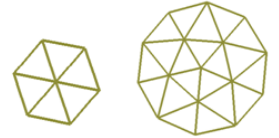
\includegraphics[width=10cm]{images/Curvature/OneRingNeighborhood}
    \end{center}
    \caption[$1$-voisinage et $2$-voisinage.]{$1$-voisinage de valence $6$ et
    $2$-voisinage de valence $5$ (Figure~1 de \cite{Gatzke2006}).}
    \label{fig:one-ring-neighborhood}
\end{figure}

Globalement, nous pouvons les distinguer en trois catégories :
\begin{itemize}
  \item Méthode par Correspondance
  \item Méthodes discrètes
  \item Estimation du tenseur de courbure
\end{itemize}

\cauthors{Surazhsky}{Surazhsky2003} et \cauthors{Gatzke}{Gatzke2006} ont par
ailleurs proposé une comparaison compréhensible de ces estimateurs. Nous nous
référons à \cauthors{Desbrun}{Desbrun2005} et \cauthors{Bobenko}{Bobenko2008}
pour une théorie entièrement discrète. Cependant, la plupart n'ont aucunes
garanties de convergence théorique des valeurs estimées, même sans bruit sur le
maillage. Nous pouvons citer \cite{Page2002} et \cite{Rusinkiewicz2004} comme
approches qui essayent de plaquer les perturbations sur la surface à travers un
moyennage.

\cauthor{Xu}{Xu2006} estime la courbure gaussienne avec une
approche dérivée de la formule de Gauss-Bonnet (défaut d'angle) et donne un
théorème de stabilité pour les maillages triangulés dont les sommets épousent la
variété lisse sous-jacente, de valence $6$, et respectant les conditions d'un
parallélogramme (tous le $1$-voisinage sont projetés comme un parallélogramme
sur un plan). En assumant que la densité de l’échantillonnage est $\delta$,
\nauthor{Xu} propose une propriété de convergence supplémentaire lorsque
l'échantillonnage est perturbé par une erreur $O(\delta^\alpha)$, mais avec
$\alpha > 2$ (ce qui est inapproprié pour des données discrètes car ce sont des
outliers). \todoJeremy{détailler plus en détail ($>\_<$), avec formules et
schéma} Il est à noter que si le maillage triangulé ne satisfait pas ces
conditions, l'estimation ne converge pas.

Une autre approche notable est l'estimation d'information de
courbure par intégration de mesures des courbures, basée sur la théorie du cycle
des normales \cite{CohenSteiner2003,CohenSteiner2006} sur un maillage triangulé.
Les auteurs (\nauthors{Cohen-Steiner}) mettent en avant des résultats de
convergence lorsque les sommets épousent le bord de l'objet euclidien
sous-jacent. Dans ce cas, si le maillage a une distance de Hausdorff avec le
bord de la forme au dessous de $\epsilon$, la convergence peut être obtenue avec
une vitesse/erreur en $O(\epsilon)$ sous certaines conditions.
\todoJeremy{détailler}

Enfin, en \emph{traitement géométrique}, d'intéressants outils
mathématiques ont été développés pour concevoir des estimateurs différentiels
sur des surfaces lisses basées sur les invariants par intégration
(\cauthors{Pottmann}{Pottmann2007,Pottmann2009}). Cela consiste à faire déplacer
une boule le long de la surface de la forme et calculer des intégrales sur
l'intersection entre la forme et la boule. Les auteurs ont démontrés que ces
quantités par intégration apportent d'intéressantes informations de courbure
lorsque la taille de la boule tend vers zéro. Ils amènent également des preuves
de stabilité --- dans le cas d'échantillonnage de maillage par exemple ---
dépendant de la taille de la boule et du $\epsilon$. Nos travaux sur les
estimateurs digitaux de courbure se basent sur la même idée.

\subsubsection{Estimation de courbure sur des nuages de points}

Lorsque nous avons des données discrètes (par exemple un nuage de points), la
façon la plus naturelle d'approcher la courbure est de faire correspondre une
surface polynomiale de degré $2$ ou plus. Le meilleur représentant de cette
technique est les « \anglais{Osculating jets} » de
\cauthors{Cazals}{Cazals2005}. Les auteurs proposent des résultats de
convergence en $O(\delta^2)$ lorsque la donnée d'entrée est un échantillonage de
la surface, avec $\delta$ la densité de points. Cependant, lorsque les données
présentent du bruit, aucun résultat théorique n'est apporté malgré qu'en
pratique la correspondance aux moindres carrés des jets osculatoires est très
robuste.

Une autre famille de techniques utilisent le diagramme de Voronoi
\cite{Alliez2007,Merigot2009,Merigot2011}. L'idée principale derrière cette
approche est qu'au lieu de faire des correspondances dans l'espace tangent à la
surface, d'estimer au mieux dans l'espace orthogonal. La mesure de covariance
convoluée introduite par \cauthors{Mérigot}{Merigot2011} est particulièrement
intéressante car cette mesure apporte de la robustesse même pour des ensembles
compacts arbitraires, en $O(\sqrt{\epsilon})$. C'est en quelque sorte la mesure
intégrale de la matrice de covariance du cône de normale autour du point
d'intérêt. Néanmoins, la convergence des courbures est dépendante de plusieurs
paramètres $r$ et $R$ qui contribuent de manière contradictoire avec l'erreur de
Hausdorff. En pratique, cette approche donne des résultats comparables aux jets
osculatoires pour les courbures.

Récemment, plusieurs auteurs ont développés de nouvelles approches intéressantes
pour estimer les champs de normales sur des nuages de points bruités, même en
présence de singularités \cite{Li2010, Boulch2012, Zhang2013}.
\cauthors{Boulch}{Boulch2012} apportent également des résultats de convergence
probabilistes. Cependant, ces méthodes ne peuvent pas être utilisées « telles
quelles » pour le calcul de coubure : ils peuvent être utilisées en parallèle
avec des techniques d'estimation de coubure pour détecter les singularités sur
la surface dans un premier temps, et de limiter l'estimation de la courbure aux
zones lisses.

\subsubsection{Estimation de courbure sur des surfaces digitales}

Comme vu dans le \RefChapitre{sec:notions}, en géométrie digitale nous
considérons généralement la convergence asymptotique comme un critère essentiel
pour un estimateur \cite{Coeurjolly_ChapEstimateur}. En dimension 2, des
résultats de convergence d'estimateurs sans paramètres ont été obtenus pour
l'estimation de longueur \cite{dcoeurjo_length_PAMI} et des normales
\cite{deVieilleville2007}.

Basés sur des principes de convolutions binomiales
\cite{MalgouyresBF08,Esbelin2011}, ou sur la correspondance de surface
polynomiales \cite{Provot11}, des résultats de convergence peuvent être obtenus
pour les dérivés d'ordre supérieurs de courbes digitales. Ces algorithmes sont
paramétrisés par la taille de la convolution ou le support du kernel utilisé
pour la correspondance, et les théorèmes de convergence \todoJeremy{trouve plus
les mots, nécessite, a besoin} quand la taille de support est une fonction
croissante de la résolution de la grille et de quelques caractéristiques de la
forme à estimer.

Pour l'estimation de courbure le long de courbes 2D, la convergence asymptotique
d'estimateurs ne nécessitant aucuns paramètres représente toujours un défi
%
% For curvature estimation along 2D curves, multigrid convergence of
% parameter-free \comJeremy{estimators} is still challenging, although accurate
% experimental results have been obtained with maximal digital circular
% arcs \cite{Roussillon11} and with global optimization
% \cite{Kerautret:2009-pr}. In 3D digital space, several empirical
% methods exist for estimating curvatures, but none achieves multigrid
% convergence (e.g. see \cite{Lenoir:1997-dgci,Fourey08}). In
% \cite{dgci2013II}, we recently presented a digital estimator for mean
% curvature for 2D and 3D digital objects, which achieves multigrid
% convergence in $O(h^{\frac{1}{3}})$.

\todoInlineJeremy{finir}
\todoJeremy{J'aurais parlé de la convergence avant, donc inutile de redire ici.}
\subsection{Estimation de la courbure par intégration volumique de la sphère}
\label{sec:estimators:volume}
%
En \GeometryProcessing, les invariants par intégration ont été largement
étudiées pour définir des estimateurs de quantités différentielles.
\cauthors{Pottmann}{Pottmann2007,Pottmann2009} en ont d'ailleurs fait une vue
d'ensemble complète. L'idée principale est de déplacer un noyau sur les points
$\vx \in \dS$ et calculer l'intégrale de l'intersection entre $\Shape$ et le
noyau. Différents noyaux peuvent être considérés (sphère euclidienne, boule
euclidienne) ainsi que différentes fonctions d'intégration (linéaire,
gaussienne, etc.). Nous n'utiliserons par la suite que les invariants volumiques
par intégration définis tels que :
\begin{definition}\label{def:Volume}
  Pour une forme $\Shape \in \Shapes$ et un rayon $R \in \R^{+*}$, l'intégrale
  volumique $V_R(\vx)$ au point $\vx \in \dS$ est donné par :
  \begin{equation}
    V_R(\vx) \EqDef \int_{\Ball{R}{\vx}}  \chi(p)dp\,,
  \end{equation}
  où $\Ball{R}{\vx}$ est une boule euclidienne de rayon $R$ et de centre $\vx$, et
  $\chi(p)$ est la fonction caractéristique de $\Shape$. En dimension 2, nous
  noterons cette quantité $A_R(\vx)$.
\end{definition}
%
\subsubsection{Analyse euclidienne de l'intégration volumique de la sphère, et relation à la courbure}
%
La relation entre $A_R(\vx)$ et la courbure (\resp $V_R(\vx)$ et la courbure
moyenne ) au point $\vx$ pour des formes de $\R^2$ (\respp $\R^3$) a beaucoup
été étudiée \cite{Bullard1995,Pottmann2007,Pottmann2009}, ainsi, nous pouvons la
formaliser de la sorte :
%
\begin{lemma}{\textbf{\cite{Pottmann2009}}}\\
\label{lem:pottmann-2d}
  Pour une forme suffisamment lisse\footnote{éclaircir} $\Shape$ de $\R^2$, $\vx
  \in \dS$, nous avons :
  \begin{equation}
    \label{eq:volume2d}
    A_R(\vx) = \frac{\pi}{2} R^2 - \frac{\Curv(\Shape,\vx)}{3}R^3 + O(R^4)\,.
  \end{equation}
  où $\Curv(\Shape,\vx)$ est la courbure de $\dS$ au point $\vx$.

  Pour une forme suffisamment lisse\footnote{éclaircir} $\Shape$ de $\R^3$, $\vx
  \in \dS$, nous avons :
  \begin{equation}
    \label{eq:volume3d}
    V_R(\vx) = \frac{2\pi}{3} R^3 - \frac{\pi \MeanCurv(\Shape,\vx)}{4}R^4 + O(R^5)\,.
  \end{equation}
  où $\MeanCurv(\Shape,\vx)$ est la courbure moyenne de $\dS$ au point $\vx$.
\end{lemma}
%
De tels résultats sont obtenus par approximation de Taylor au point $\vx$ de la
surface $\dS$ approximée par la fonction paramtétrique $z=f(x,y)$ ($y=f(x)$ en
2D). Alors, des \RefEquations{eq:volume2d}{eq:volume3d}, avec un
rayon $R$ fixé, nous pouvons définir les estimateurs locaux de coubure 2D
$\CurvT{R}(\vx)$ et de courbure moyenne 3D $\MeanCurvT{R}(\vx)$.
%
\begin{definition}{\textbf{(Estimateurs de courbure 2D $\CurvT{R}(\Shape,\vx)$ et de courbure moyenne 3D $\MeanCurvT{R}(\Shape,\vx)$ \cite{Pottmann2007}).}}
  \label{def:pottmann-2d-3d-mean}
  Pour une forme $\Shape \subset \R^2$, l'estimateur de courbure 2D $\CurvT{R}$
  au point $\vx \in \dS$ est défini par :
  \begin{equation}
    \label{eq:pottmann-2d}
    \CurvT{R}(\Shape,\vx) \EqDef \frac{3\pi}{2 R} - \frac{3 A_R(\vx)}{R^3},
  \end{equation}

  Pour une forme $\Shape \subset \R^3$, l'estimateur de courbure moyenne 3D
  $\MeanCurvT{R}$ au point $\vx \in \dS$ est défini par :
  \begin{equation}
    \label{eq:pottmann-3d-mean}
    \MeanCurvT{R}(\Shape,\vx) \EqDef \frac{8}{3 R} - \frac{4 V_R(\vx)}{\pi R^4}.
  \end{equation}
\end{definition}
%
De plus, lorsque me rayon $R$ tend vers zéro, les valeurs de ces deux
estimateurs vont converger vers celles espérées. Plus formellement :
%
\begin{theorem}{\textbf{(Convergence des estimateurs de courbure 2D $\CurvT{R}(\Shape,\vx)$ et de courbure moyenne 3D $\MeanCurvT{R}(\Shape,\vx)$ \cite{Pottmann2007}).}}
  \label{theo:pottmann-2d-3d-mean-conv}
  \begin{equation}
    \CurvT{R}(\Shape,\vx) = \Curv(\Shape,\vx) + O(R),
    \quad\MeanCurvT{R}(\Shape,\vx) = \MeanCurv(\Shape,\vx) + O(R).
  \end{equation}
\end{theorem}
%
De la même manière, des informations directionnelles comme les courbures
principales (et donc la courbure gaussienne) peuvent être extraitent du calcul
par intération. En effet, à la place de calculer la mesure de $\Ball{R}{\vx}$ dans
la \RefDefinition{def:pottmann}, nous allons calculer sa matrice de covariance.
%
\begin{definition}
  \label{def:cov-matrix}
  Pour un ensemble non vide $Y \subset \R^d$, la matrice de covariance de $Y$
  est définie par :
  \begin{equation}
    \Cov(Y) \EqDef \int_Y (\vp-\overline{Y})(\vp-\overline{Y})^T d\vp = \int_Y \vp \vp^T d\vp - \Vol(Y)\overline{Y}\overline{Y}^T,
  \end{equation}
  où $\overline{Y}$ est le barycentre de $Y$ et $\Vol(Y)$ son volume.
\end{definition}
%
Pour les entiers $p, q, s \ge 0$, nous pouvons écrire la définition des $
pqs$-moments $\Mom{pqs}(Y)$ de $Y$ ($x_i$ est la $i$ème composante de $\vx$) :
%
\begin{equation}
  \label{eq:moments}
  \Mom{pqs}(Y) \EqDef \iiint_Y x_1^p x_2^q x_3^s dx_1 dx_2 dx_3\,.
\end{equation}
%
Il apparaît alors clairement que le volume $\Vol(Y)$ est le $0$-moment
$\Mom{000}(Y)$, et que le barycentre $\overline{Y}$ est le $1$-moment normalisé
par le $0$-moment, c'est à dire :
%
\begin{equation}
  \overline{Y} \EqDef \frac{( \Mom{100}(Y), \Mom{010}(Y), \Mom{001}(Y) )^T}{\Mom{000}(Y)}
\end{equation}
%
\begin{lemma}\label{lem:moment-ball}
  %
  Soit $\Ball{R}{\vx}$ une boule de rayon $R$ et de centre $\vy$. Alors, pour un
  ensemble non vide $Y \subset \Ball{R}{t}$, nous avons :
  %
  \begin{align}
    \Mom{000}(Y) =& O(R^3), \label{eq:ball-moment-0}\\
    \Mom{100}(Y) =& O(R^3(\|\vy\|_\infty + R)), \label{eq:ball-moment-1}\\
    \Mom{200}(Y) =& O(R^3(\|\vy\|^2_\infty + R\|\vy\|_\infty + R^2)), \label{eq:ball-moment-2}\\
    \Mom{100}(Y)/\Mom{000}(Y) =& O(R+\vy), \label{eq:ball-moment-1bis}
  \end{align}
  %
  Les autres moments du même ordre ont respectivement les mêmes bornes.
  %
\end{lemma}
\begin{proof}
  %
  \textbf{Moment d'ordre zéro.\quad}
  %
  L'\RefEquation{eq:ball-moment-0} peut être facilement démontré puisque le
  moment d'ordre zéro est le volume de $Y$, de ce fait ne peut pas dépasser le
  volume de la boule qui est $\frac{4}{3}\pi R^3$.
  %
  \textbf{\\Moments du premier ordre.\quad}
  %
  Nous changeons les variables de $(x_1',x_2',x_3')=(x_1,x_2,x_3)-\vy$ dans
  l'expression suivante :
  %
  \begin{align}
    \Mom{100}(Y) &= \iiint_Y x_1 dx_1 dx_2 dx_3 = \iiint_{Y-\vy} (x_1'+y_1) dx_1'dx_2'dx_3' \\
                 &= y_1 \Vol(Y) + \Mom{100}(Y-\vy).
  \end{align}
  %
  Dans le premier terme, $\Vol(Y)$ est borné par le volyme de la boule de rayon
  $R$. Avec la propriété d'additivité des intégrales, le second terme est
  maximisé par le $100$-moment de la demi-boule $\HalfBall{R}{0}$ centrée en $0$ à
  valeur de $x_1$ positives. Alors, en utilisant les coordonnées sphériques,
  nous obtenons :
  %
  \begin{align}
    \Mom{100}(\HalfBall{R}{0})
    &= \int_{0}^{R} \int_{\frac{-\pi}{2}}^{\frac{\pi}{2}} \int_{\frac{-\pi}{2}}^{\frac{\pi}{2}} (\rho\cos\phi\cos\theta)(\rho^2 \cos\phi)  \, d\theta d\phi d\rho \\
    &= \left[\frac{\rho^4}{4} \right]_{0}^{R}  \left [\sin\theta\right ]^\frac{\pi}{2}_{-\frac{\pi}{2}}\frac{1}{2} [\phi + \sin(\phi)\cos(\phi)]^\frac{\pi}{2}_{-\frac{\pi}{2}} \\
    &= \frac{\pi}{4}R^4, \label{eq:exact-half-ball-moment-1}
  \end{align}
  %
  Les autres équations sont prouvées de la même façon.
  %
\end{proof}
%
Pour plus de simplicité dans les formules, nous noterons $A$ l'ensemble
euclidien $\Ball{R}{\vx} \cap \Shape$. La matrice de covariance $\Cov(A)$ de
$A$ peut alors être réécrite comme :
\begin{align}
  \Cov(A) &=  \left\lbrack
    \begin{array}{ccc}
      \Mom{200}(A) & \Mom{110}(A) & \Mom{101}(A)\\
      \Mom{110}(A) & \Mom{020}(A) & \Mom{011}(A)\\
      \Mom{101}(A) & \Mom{011}(A) & \Mom{002}(A)
    \end{array}
    \right\rbrack\quad\quad\quad\quad\quad\quad \nonumber \\
    &\quad\quad\quad\quad\quad\quad- \frac{1}{\Mom{000}(A)}
    \left\lbrack
    \begin{array}{c}
      \Mom{100}(A) \\
      \Mom{010}(A) \\
      \Mom{001}(A) \\
    \end{array}
    \right\rbrack
    \otimes
    \left\lbrack
    \begin{array}{c}
      \Mom{100}(A) \\
      \Mom{010}(A) \\
      \Mom{001}(A) \\
    \end{array}
    \right\rbrack^T.
\label{eq:defCov}
\end{align}
%
où $\otimes$ désigne le produit de tensoriel dans l'espace des vecteurs.
%
\cauthors{Pottmann}{Pottmann2007} ont démontré que les valeurs propres et les
vecteurs propres de $\Cov(A)$ fournissaient des informations sur les courbures
principales et directions principales de courbure :
\begin{lemma}[\cite{Pottmann2007}, Théorème~2]
 \label{lem:pottmann-3d}
 Pour une forme $\Shape \in \Shapes$, les valeurs propres $\lambda_1$,
 $\lambda_2$, $\lambda_3$ de $\Cov(A)$, où $ A \EqDef \Ball{R}{\vx} \cap
 \Shape$ et $\vx \in \Bd{\Shape}$, $\lambda_1 \ge \lambda_2 \ge
 \lambda_3$, nous avons l'approximation de Taylor suivante :
 \begin{align}
   \lambda_1& = \frac{2\pi}{15}R^5 - \frac{\pi}{48}(3\PrincCurv{1}(\Shape,\vx) + \PrincCurv{2}(\Shape,\vx))R^6 + O(R^7)\,,\\
   \lambda_2& = \frac{2\pi}{15}R^5 - \frac{\pi}{48}(\PrincCurv{1}(\Shape,\vx) + 3\PrincCurv{2}(\Shape,\vx))R^6 + O(R^7)\,,\\
   \lambda_3& = \frac{19\pi}{480}R^5 - \frac{9\pi}{512}(\PrincCurv{1}(\Shape,\vx) + \PrincCurv{2}(\Shape,\vx))R^6 + O(R^7)\,,
 \end{align}
 où $\PrincCurv{1}(\Shape,\vx)$ et $\PrincCurv{2}(\Shape,\vx)$ désignent les
 courbures principales de  $\Bd{\Shape}$ au point $\vx$.\footnote{Il y a une
 erreur typographique dans l'expression de $\lambda_1$ dans~\cite{Pottmann2007}.}
\end{lemma}
%
De même qu'avec l'\RefEquation{def:pottmann-2d-3d-mean}, nous pouvons définir
les estimateurs locaux de courbures principales $\PrincCurvT{1}{R}$ et
$\PrincCurvT{2}{R}$ et de courbure gaussienne $\GaussCurvT{R}$ comme des
fonctions de $\{\lambda_i\}_{1,2,3}$ et de $R$ :
%
\begin{align}
  \label{eq:pottmann-3d-princ}
  \PrincCurvT{1}{R}(\Shape,\vx)& \EqDef \frac{6}{\pi R^6}(\lambda_2 - 3\lambda_1) + \frac{8}{5R}\,,\\
  \PrincCurvT{2}{R}(\Shape,\vx)& \EqDef \frac{6}{\pi R^6}(\lambda_1 - 3\lambda_2) + \frac{8}{5R}\,,\\
  \GaussCurvT{R}(\Shape,\vx)& \EqDef \PrincCurvT{1}{R} \cdot \PrincCurvT{2}{R}.
\end{align}
%
D'après le \RefLemma{lem:pottmann-3d}, tous ces estimateurs approchent la
quantité espérée lorsque le rayon $R$ tend vers $0$ :
%
\begin{align}
  \label{eq:pottmann-3d-princ}
  \PrincCurvT{1}{R}(\Shape,\vx)& = \PrincCurv{1}(\Shape,\vx) + O(R)\,,\\
  \PrincCurvT{2}{R}(\Shape,\vx)& = \PrincCurv{2}(\Shape,\vx) + O(R)\,,\\
  \GaussCurvT{R}(\Shape,\vx)& = \GaussCurv(\Shape,\vx) + ???.
\end{align}
\todoJeremy{vérifier !!!!}
%
Lorsque nous nous intéressons à des formes digitales $\AnyDSh$, l'implémentation
de ces estimateurs devient direct : choisir un rayon $R$, centrer une boule
euclidienne (ou digitale) sur des points de $\Bd{\Body{\AnyDigF{\Shape}{h}}{h}}$
(\cad les barycentres de linels en 2D ou surfels en 3D)\todoJeremy{Confirmer
surfel = 3D ?}, calculer la quantité (aire, volume ou matrice de covariance) et
enfin estimer l'information de courbure $\CurvT{R}$, $\MeanCurvT{R}$,
$\PrincCurvT{1}{R}$, $\PrincCurvT{2}{R}$ or $\GaussCurvT{R}$.
%
Cependant, quelques problèmes surviennent dans cette approche : comment bien
estimer l'aire, le volume ou la matrice de covariance sur des formes digitales,
pouvons nous conclure à des preuves de convergence des estimateurs sur des
données digitales et que veut dire « $R$ tend vers zéro » quand la taille de la
grille digitale influe également dessus ? Dans une premier temps nous allons
nous intéresser à l'aire et au volume digital, puis dans un second temps aux
moments digitaux.
%
\subsubsection{Analyse digitale de l'aire et du volume de la sphère, et relation à la courbure}
%
Nous souhaitons estimer la quantité $A_R(\vx) = \Area(\Ball{R}{\vx}\cap\Shape)$ de la
\RefDefinition{def:Volume} au pas de discrétisation $h$, où $\Ball{R}{\vx}$ est une
boule de rayon $R$ centrée au point $\vx$. Nous ne pouvons pas directement
utiliser les résultats des
\RefEquations{eq:AreaByCountingConv}{eq:VolumeByCountingConv} pour estimer cette
aire : le terme d'erreur en grand « O » cache le fait que la constante impliquée
dépend de la taille de la forme, son échelle et sa courbure maximale. Un moyen
simple de comprendre cet effet en estimant l'aire d'une forme $\Shape$ et
d'estimer l'aire de la même forme doublée en taille (que nous nommerons
$\Shape'$). Alors, il paraît évident que :
%
\begin{equation}
  2 \cdot \AreaC(\DSh,h) \ne \AreaC(\DigF{\Shape'}{h},h),
\end{equation}
%
la discrétisation de $\Shape'$ le rendant plus détaillé et donc son estimation
plus précise. C'est un problème génant avec les invariants par intégration car
les boules impliquées ont un rayon $R$ qui doit tendre vers $0$ lorsque $h$ tend
également vers $0$. Nous devons alors normaliser notre estimation d'aire et de
volume pour que le terme d'erreur ne soit plus influencé par l'échelle de la
boule. Nous estimons alors l'aire de l'intersection entre la forme et la boule
de rayon $R$ en se ramenant à la boule unité :
%
\begin{align}
  \AreaC(\DigF{\Ball{R}{\vx} \cap \Shape}{h}, h) & \EqDef h^2 \MCard( ( \frac{1}{h} \cdot ( \Ball{R}{\vx} \cap \Shape ) ) \cap \Z^2 ), \\
   & = h^2 \MCard( (\frac{R}{h} \cdot ( \Ball{1}{\frac{1}{R} \cdot \vx} \cap \frac{1}{R} \cdot \Shape) ) \cap \Z^2 ), \\
   & = R^2 \frac{h^2}{R^2} \MCard( (\frac{R}{h} \cdot ( \Ball{1}{\frac{1}{R} \cdot \vx} \cap \frac{1}{R} \cdot \Shape) ) \cap \Z^2 ), \\
   & = R^2 \AreaC( \DigF{\Ball{1}{\frac{1}{R} \cdot \vx} \cap \frac{1}{R} \cdot \Shape}{h/R}, h/R ), \label{eq:Area_unitary_ball}
\end{align}
%
Alors, en insérant l'\RefEquation{eq:AreaByCountingConv} dans le terme de droite
de \ref{eq:Area_unitary_ball}\footnote{Le terme $\beta$ est celui défini dans le \RefSection{sec:AreaByCounting}.} :
\begin{equation}
  \label{eq:Area_unitary_ball_shape}
  \AreaC(\DigF{\Ball{R}{\vx} \cap \Shape}{h}, h) = R^2 \left(\Area( \Ball{1}{\frac{1}{R} \cdot \vx} \cap \frac{1}{R} \cdot \Shape) + O( (h/R)^\beta) \right).
\end{equation}
%
Notons $SB(R)$ l'ensemble $\Ball{1}{\frac{1}{R} \cdot \vx} \cap \frac{1}{R} \cdot
\Shape$. La constante $K_1$ associée au terme d'erreur grand « O » dépend
uniquement de la courbure maximale de $\BT SB(R)$. La courbure n'est pas définie
aux intersections des deux bords de la forme et de la boule (dans le
sous-ensemble $\BT \Ball{1}{\frac{1}{R} \cdot \vx} \cap \frac{1}{R} \cdot \dS$) mais
son influence dans l'estimation d'aire est négligeable car au moins de l'ordre
de $O(h^2)$. La partie restante de $\BT SB(R)$ a une courbure maximale qui est
égale à $1$ pour un rayon $R$ suffisamment petit. En effet, puisque $\Shape$ a
une courbure bornée, son dilaté $\frac{1}{R} \cdot \dS$ devient plat au point
$\frac{1}{R} \cdot \vx$, alors la courbure maximale est introduite par $\BT
\Ball{1}{\vx}$. Nous pouvons conclure qu'il existe quelques rayons $R_0$ tels que la
constante $K_1$ intervient pour un rayon arbitraire $R < R_0$. En développant le
terme d'erreur en grand « O » avec $K_1$, et en insérant dans
l'\RefEquation{eq:Area_unitary_ball_shape} la relation :
%
\begin{equation}
  A_R(\vx) = \Area( \Ball{R}{\vx} \cap \Shape ) = R^2 \Area( \Ball{1}{\frac{1}{R} \cdot \vx} \cap \frac{1}{R} \cdot \Shape),
\end{equation}
%
nous obtenons :
%
\begin{equation}\label{eq:convergence-area-intersection}
  | \AreaC(\DigF{\Ball{R}{\vx} \cap \Shape}{h}, h) - A_R(\vx) | \le K_1 h^\beta R^{2-\beta}.
\end{equation}
%
La convergence de la précédente relation tient du fait que $h \le R \le R_0$ et
est valide quand $\vx$ est n'importe quel point de $\R^2$ (pas seulement un
point de $\dS$). De plus, la constante $K_1$ est indépendante de la forme
$\Shape$ (mais dépendante de $R_0$).\\
%
Le même raisonnement est valide en dimension 3 : la courbure n'est alors pas
définie dans le sous-ensemble $\BT \Ball{1}{\frac{1}{R} \cdot \vx} \cap \frac{1}{R}
\cdot \dS$, qui tend vers le cercle unité lorsque $R \rightarrow 0$. L'erreur
introduite dans l'estimation de volume est alors le nombre de voxels intersectés
($\approx 2\pi/h$), ce qui est négligeable. La courbure maximale est également
$1$ pour un rayon $R$ suffisement petit. Nous obtenons alors :
%
\begin{equation}\label{eq:convergence-volume-intersection}
  | \VolC(\DigF{\Ball{R}{\vx} \cap \Shape}{h}, h) - V_R(\vx) | \le K_1 h^\gamma R^{3-\gamma}.
\end{equation}
%
\paragraph{Estimateurs digitaux de courbure 2D et de courbure moyenne 3D par intégration}
%
Nous allons définir des estimateurs digitaux de courbure 2D $\CurvH{R}$ et de
courbure moyenne 3D $\MeanCurvH{R}$ dans le même esprit que la
\RefDefinition{def:pottmann-2d-3d-mean}, auxquels le calcul consiste uniquement à
compter le nombre de points digitaux dans un voisinage du point d'intérêt :
%
\begin{figure}[ht]
  \begin{center}
    
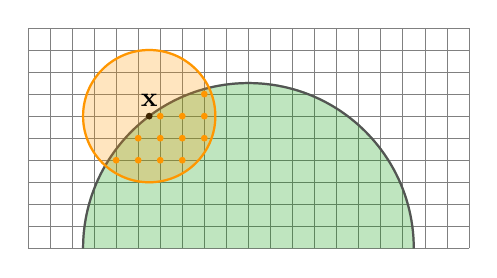
\begin{tikzpicture}[x=0.28cm,y=0.28cm]
  % colors
  \definecolor{kGreen}{rgb}{0.0,0.59,0.0}
  \definecolor{kOrange}{rgb}{1.0,0.59,0.0}
  \definecolor{kGrey}{rgb}{0.33,0.33,0.33}
  % grids
  \draw[help lines,step=1] (0,0) grid (20,10);
  \draw[draw,thick,fill,color=kGreen,nearly transparent] (2.5,0) arc (180:0:7.5);
  \draw[draw,thick,color=kGrey] (2.5,0) arc (180:0:7.5);
  \node (px) at (5.5,6) {};
  \draw[draw,thick,color=black,fill] (px) circle (0.1);
  \draw[draw,thick,fill,color=kOrange,nearly transparent] (px) circle (3);
  \draw[draw,thick,color=kOrange] (px) circle (3);
  \draw (px) node[above] {$\mathbf{x}$};
  \foreach \x/\y in {4/4, 5/4, 6/4, 7/4, 5/5, 6/5, 7/5, 8/5, 6/6, 7/6, 8/6, 8/7}
    \draw[draw,thick,color=kOrange,fill] (\x,\y) circle (0.1);
\end{tikzpicture}
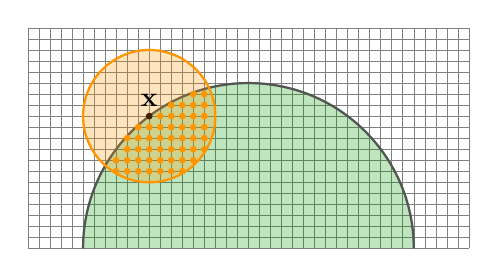
\begin{tikzpicture}[x=0.28cm,y=0.28cm]
  % colors
  \definecolor{kGreen}{rgb}{0.0,0.59,0.0}
  \definecolor{kOrange}{rgb}{1.0,0.59,0.0}
  \definecolor{kGrey}{rgb}{0.33,0.33,0.33}
  % grids
  \draw[help lines,step=0.5] (0,0) grid (20,10);
  \draw[draw,thick,fill,color=kGreen,nearly transparent] (2.5,0) arc (180:0:7.5);
  \draw[draw,thick,color=kGrey] (2.5,0) arc (180:0:7.5);
  \node (px) at (5.5,6) {};
  \draw[draw,thick,color=black,fill] (px) circle (0.1);
  \draw[draw,thick,fill,color=kOrange,nearly transparent] (px) circle (3);
  \draw[draw,thick,color=kOrange] (px) circle (3);
  \draw (px) node[above] {$\mathbf{x}$};
  % line 3.5
  \foreach \x in {4, 4.5, 5, 5.5, 6, 6.5, 7}
    \draw[draw,thick,color=kOrange,fill] (\x,3.5) circle (0.1);
  % line 4
  \foreach \x in {4, 4.5, 5, 5.5, 6, 6.5, 7, 7.5}
    \draw[draw,thick,color=kOrange,fill] (\x,4) circle (0.1);
  % line 4.5
  \foreach \x in {4.5, 5, 5.5, 6, 6.5, 7, 7.5, 8}
    \draw[draw,thick,color=kOrange,fill] (\x,4.5) circle (0.1);
  % line 5
  \foreach \x in {4.5, 5, 5.5, 6, 6.5, 7, 7.5, 8}
    \draw[draw,thick,color=kOrange,fill] (\x,5) circle (0.1);
  % line 5.5
  \foreach \x in {5, 5.5, 6, 6.5, 7, 7.5, 8}
    \draw[draw,thick,color=kOrange,fill] (\x,5.5) circle (0.1);
  % line 6
  \foreach \x in {6, 6.5, 7, 7.5, 8}
    \draw[draw,thick,color=kOrange,fill] (\x,6) circle (0.1);
  % line 6.5
  \foreach \x in {6.5, 7, 7.5, 8}
    \draw[draw,thick,color=kOrange,fill] (\x,6.5) circle (0.1);
  % line 7
  \foreach \x in {7.5, 8}
    \draw[draw,thick,color=kOrange,fill] (\x,7) circle (0.1);
\end{tikzpicture}

  \end{center}
  \caption[Illustration de l'estimateur digital de courbure 2D par intégration
  $\CurvH{R}$.]{Illustration de l'estimateur digital de courbure 2D par
  intégration $\CurvH{R}$ avec deux pas de discrétisation de la forme $h$
  différents.\label{fig:2d-curv-estimator}}
\end{figure}
%
\begin{definition}[Estimateur digital de courbure 2D par intégration.]\label{def:digital-2d-curvature}
  %
  Pour tout rayon $R$ positif, nous définissons l'estimateur digital de courbure
  2D par intégration $\CurvH{R}$ d'une forme digitale $\DigShape \subset \Z^2$
  en tout point $\vx \in \R^2$ et pour le pas de discrétisation $h > 0$ comme :
  %
  \begin{equation}
    \forall 0 < h < R,\quad \CurvH{R}(\DigShape,\vx,h) \EqDef \frac{3\pi}{2R} - \frac{3\AreaC(\Ball{R/h}{\vx/h} \cap \DigShape, h)}{R^3}\,.
  \end{equation}
  %
\end{definition}
%
\begin{definition}[Estimateur digital de courbure moyenne 3D par intégration.]
  %
  Pour tout rayon $R$ positif, nous définissons l'estimateur digital de courbure
  moyenne 3D par intégration $\MeanCurvH{R}$ d'une forme digitale $\DigShape
  \subset \Z^3$ en tout point $\vx \in \R^3$ et pour le pas de discrétisation $h >
  0$ comme :
  %
  \begin{equation}
    \forall 0 < h < R,\quad \MeanCurvH{R}(\DigShape,\vx,h) \EqDef \frac{8}{3R} - \frac{4\VolC(\Ball{R/h}{\vx/h} \cap \DigShape, h)}{\pi R^4}\,.
  \end{equation}
  %
\end{definition}
%
Comme le montre la \RefFigure{fig:2d-curv-estimator}, ces estimateurs placent
une boule de rayon euclidien $R$ autour du point d'intérêt $\vx$ et comptent le
nombre de points digitaux de $\DigShape$, après mise à l'échelle en $(h\Z)^d$,
de l'intersection de cette boule et de la forme. Un calcul linéaire simple est
alors appliqué sur cette quantité afin d'approximer la courbure. De plus, comme
le montre également la \RefFigure{fig:2d-curv-estimator}, nous pouvons supposer
que si la discrétisation s'affine nous aurons une meilleure estimation de la
courbure. Le prochain paragraphe va le démontrer.
%
\paragraph{Convergence des estimateurs digitaux de courbure 2D et de courbure moyenne 3D par intégration}
%
Nous allons ici montrer que les estimateurs de courbure 2D $\CurvH{R}$ et de
courbure moyenne 3D $\MeanCurvH{R}$ convergent vers la valeur espérée de
courbure pour tous les points $\vx$ le long du bord $\dS$ de l'objet $\Shape$ si
la forme respecte certaines contraintes.\\
%
\begin{theorem}[Convergence de l'estimateur digital de courbure 2D $\CurvH{R}$ le long de $\dS$.]
  \label{thm:convergence-curv-2d}
  %
  Soit $\Shape$ un domaine compact de $\R^2$ tel que son bord $\dS$ est $C^2$ et
  sa courbure bornée. Alors, l'estimateur digital de courbure 2D $\CurvH{R}$ en
  tout point $\vx$ de $\dS$ converge vers la courbure
  $\Curv(\Shape,\vx)$ de $\Shape$ au point $\vx$ pour la discrétisation de
  Gauss, avec une vitesse de convergence d'au moins $O(h^{\frac{1}{3}})$ lorsque
  $R = O(h^{\frac{1}{3}})$. Plus précisement, nous avons :
  %
  \begin{equation}
    \forall 0 < h < h_0,
    \quad \left | \CurvH{R}(\DSh, \vx, h) - \Curv(\Shape, \vx) \right|
                          \le O \left(h^{\frac{1}{3}}\right). %% O(R) + K_1 R h.
  \end{equation}
  %
\end{theorem}
\begin{proof}
  %
  En utilisant les relations sur les invariants par intégration définis
  précédement (\RefDefinition{def:digital-2d-curvature}), ainsi que la relation
  $\DigF{\Ball{R}{\vx} \cap \Shape}{h}=\Ball{R/h}{\frac{1}{h} \cdot \vx} \cap
  \DSh$, nous obtenons pour $R < R_0$ :
  %
  \begin{equation}
    | \CurvH{R}(\DSh,\vx,h) - \Curv(\Shape,\vx) |
    = \left|\frac{3\pi}{2R}-\frac{3\AreaC(\Ball{R/h}{\vx / h} \cap \DSh, h)}{R^3} - \Curv(\Shape,\vx) \right|,
  \end{equation}
  %
  en utilisant la relation entre l'estimation digitale de l'aire et l'aire
  euclidienne de l'\RefEquation{eq:convergence-area-intersection}, nous obtenons :
  %
  \begin{align}\label{eq-curvhat-error-bound-prelim}
    | \CurvH{R}(\DSh,\vx,h) - \Curv(\Shape,\vx) |
    &\le \left|\frac{3\pi}{2R}-\frac{3\Area(\Ball{R}{\vx} \cap \Shape)}{R^3} - \Curv(\Shape,\vx) \right| + 3K_1 \frac{h^\beta}{R^{1+\beta}} \nonumber \\
    &\le \left|\CurvT{R}(\Shape,\vx) - \Curv(\Shape,\vx) \right| + 3K_1 \frac{h^\beta}{R^{1+\beta}},
  \end{align}
  %
  ainsi, en utilisant le \RefTheorem{theo:pottmann-2d-3d-mean-conv}, nous pouvons
  écrire que :
  %
  \begin{equation}\label{eq-curvhat-error-bound-prelim2}
    | \CurvH{R}(\DSh,\vx,h) - \Curv(\Shape,\vx) |
    \le O(R) + 3K_1 \frac{h^\beta}{R^{1+\beta}}.
  \end{equation}
  %
  Nous obtenons alors deux termes d'erreur dépendants du rayon $R$ de la boule
  qui sont contradictoires : lorsque $R$ diminue, $O(R)$ diminue mais $3K_1
  \frac{h^\beta}{R^{1+\beta}}$ augmente, et vice-versa. Nous voulons alors
  guider le rayon $R$ afin d'obtenir un optimal de notre terme d'erreur. Nous
  proposons alors de définir $R = k h^{\alpha}$ et de choisir $k$ (une
  constante) et $\alpha$ afin de minimiser les bornes d'erreur. Nous notons
  $K_2$ la constante derrière le grand « O » de $O(R)$, nous obtenons :
  %
  \begin{equation}\label{eq-curvhat-error-bound-prelim3}
    | \CurvH{R}(\DSh,\vx,h) - \Curv(\Shape,\vx) |
    \le K_2kh^\alpha + \frac{3K_1}{k^{1+\beta}}h^{\beta - \alpha(1+\beta)}.
  \end{equation}
  %
  Alors, l'erreur minimale est atteinte lorsque les exposants sont égaux : nous
  devons résoudre $\alpha = \beta - \alpha(1+\beta)$.
  L'\RefEquation{eq:AreaByCountingConv} nous informe que $\beta = 1$ dans le cas
  général\footnote{Il est à noter que si le bord de la forme est $C^3$ sans
  courbure nulle, $\beta$ est alors égal à $\frac{15}{11} - \epsilon$ et donc
  $\alpha = \frac{15}{37} - \epsilon \approx 0.405$. Voir
  \RefSection{sec:AreaByCounting}.}, et donc $\alpha = \frac{1}{3}$. Donc,
  lorsque $R=kh^{\frac{1}{3}}$ :
  %
  \begin{align}\label{eq-curvhat-error-bound-prelim4}
    | \CurvH{R}(\DSh,\vx,h) - \Curv(\Shape,\vx) |
    &\le K_2kh^\frac{1}{3} + \frac{3K_1}{k^2}h^{\frac{1}{3}}\\
    &\le O(h^\frac{1}{3}).
  \end{align}
  %
\end{proof}
%
Nous obtenons des résultats similaires pour l'estimateur digital de courbure
moyenne sur des formes 3D :
%
\begin{theorem}[Convergence de l'estimateur digital de courbure moyenne 3D $\MeanCurvH{R}$ le long de $\dS$.]
  \label{thm:convergence-curv-3d}
  %
  Soit $\Shape$ un domaine compact de $\R^3$ tel que son bord $\dS$ est $C^3$ et
  sa courbure bornée. Alors, l'estimateur digital de courbure moyenne 3D
  $\MeanCurvH{R}$ en tout point $\vx$ de $\dS$ converge vers la
  courbure $\MeanCurv(\Shape,\vx)$ de $\Shape$ au point $\vx$ pour la
  discrétisation de Gauss, avec une vitesse de convergence d'au moins
  $O(h^{\frac{1}{3}})$ lorsque $R = O(h^{\frac{1}{3}})$. Plus précisement, nous
  avons :
  %
  \begin{equation}
    \forall 0 < h < h_0,
    \quad \left | \MeanCurvH{R}(\DSh, \vx, h) - \MeanCurv(\Shape, \vx) \right|
                          \le O \left(h^{\frac{1}{3}}\right). %% O(R) + K_1 R h.
  \end{equation}
  %
\end{theorem}
\begin{proof}
  %
  La preuve suit exactement les mêmes étapes que la preuve du
  \RefTheorem{thm:convergence-curv-2d}, la
  \RefDefinition{def:digital-3d-curvature}), ainsi que la relation
  $\DigF{\Ball{R}{\vx} \cap \Shape}{h}=\Ball{R/h}{\frac{1}{h} \cdot \vx} \cap \DSh$ nous
  permets d'obtenir pour $R < R_0$ :
  %
  \begin{equation}
    | \MeanCurvH{R}(\DSh,\vx,h) - \MeanCurv(\Shape,\vx) |
    = \left|\frac{8}{3R}-\frac{4\VolC(\Ball{R/h}{\vx / h} \cap \DSh, h)}{\pi R^4} - \MeanCurv(\Shape,\vx) \right|,
  \end{equation}
  %
  en utilisant la relation entre l'estimation digitale du volume et le volume
  euclidienne de l'\RefEquation{eq:convergence-volume-intersection}, nous obtenons :
  %
  \begin{align}\label{eq-meancurvhat-error-bound-prelim}
    | \MeanCurvH{R}(\DSh,\vx,h) - \MeanCurv(\Shape,\vx) |
    &\le \left|\frac{8}{3R}-\frac{4\Vol(\Ball{R}{\vx} \cap \Shape)}{\pi R^4} - \MeanCurv(\Shape,\vx) \right| + \frac{4 K_1}{\pi} \frac{h^\gamma}{R^{1+\gamma}} \nonumber \\
    &\le \left|\MeanCurvT{R}(\Shape,\vx) - \MeanCurv(\Shape,\vx) \right| + \frac{4 K_1}{\pi} \frac{h^\gamma}{R^{1+\gamma}},
  \end{align}
  %
  ainsi, en utilisant le \RefTheorem{theo:pottmann-2d-3d-mean-conv}, nous pouvons
  écrire que :
  %
  \begin{equation}\label{eq-meancurvhat-error-bound-prelim2}
    | \MeanCurvH{R}(\DSh,\vx,h) - \MeanCurv(\Shape,\vx) |
    \le O(R) + \frac{4 K_1}{\pi} \frac{h^\gamma}{R^{1+\gamma}}.
  \end{equation}
  %
  Comme précédemment, Les deux termes d'erreurs sont dépendants du rayon $R$ de
  la boule et ont un effet opposé, nous proposons de définir $R = k h^{\alpha}$,
  $k$ étant une constante, afin de trouver le $\alpha$ optimal pour minimiser
  l'erreur. Nous notons $K_2$ la constante derrière le grand « O » de $O(R)$,
  nous obtenons :
  %
  \begin{equation}\label{eq-meancurvhat-error-bound-prelim3}
    | \MeanCurvH{R}(\DSh,\vx,h) - \MeanCurv(\Shape,\vx) |
    \le K_2kh^\alpha + \frac{3K_1}{k^{1+\gamma}}h^{\gamma - \alpha(1+\gamma)}.
  \end{equation}
  %
  Et comme précedemment, celà revient à résoudre $\alpha = \gamma -
  \alpha(1+\gamma)$. L'\RefEquation{eq:VolumeByCountingConv} nous informe que
  $\gamma = 1$ dans le cas général\footnote{Il est à noter que si le bord de la
  forme est lisse, $\gamma$ est alors égal à $\frac{243}{158}$ et donc $\alpha =
  \frac{243}{559} \approx 0.435$. Voir \RefSection{sec:AreaByCounting}.}, et
  donc $\alpha = \frac{1}{3}$, comme en 2D. Donc, lorsque $R=kh^{\frac{1}{3}}$ :
  %
  \begin{align}\label{eq-meancurvhat-error-bound-prelim4}
    | \MeanCurvH{R}(\DSh,\vx,h) - \MeanCurv(\Shape,\vx) |
    &\le K_2kh^\frac{1}{3} + \frac{4K_1}{\pi k^2}h^{\frac{1}{3}}\\
    &\le O(h^\frac{1}{3}).
  \end{align}
  %
\end{proof}
%
Cependant, ces théorèmes ne sont valides que pour tous points $\vx$ de $\dS$.
Lorsque nous traitons des bords des surfaces digitales, une nouvelle
approximation intervient dû à la discrétisation. Le prochain paragraphe adaptera
ces estimateurs sur des contours digitaux de surface.
%
\paragraph{Convergence asymptotique pour des formes suffisamment lisses}
%
Comme nous venons de le dire, nous ne connaissont pas exactement la position de
$\vx$ lorsque nous considérons des données digitales. Les seules informations
que nous disposons sont les points digitaux $\vxH$ de $\Bd{\Body{\DSh}{h}}$.
Nous devons alors considérer l'erreur possible de positionnement de l'endroit où
est estimé la courbure pour proposer des théorèmes de convergence
asymptotiques.\\
%
Nous devons alors injecter cette approximation dans le calcul d'aire et de
volume, pour ensuite la diffuser aux calculs de courbures. Ainsi, nous pouvons
prouver la convergence asymptotique des estimateurs de courbure digitale sur le
bord digital d'un objet suffisamment lisse.
%
\begin{theorem} \label{thm:multigrid-convergence-curv}
%
Soit $\Shape$ un domaine compact de $\R^2$ tel que son bord $\dS$ est $C^3$ à
courbure bornée. Alors, l'estimateur digital de courbure $\CurvH{R}$ converge
asymptotiquement vers la courbure $\Curv$ pour la discrétisation de Gauss sur
des formes $\Shape$, avec une vitesse de convergence d'au moins
$O(h^\frac{1}{3})$ lorsque $R = kh^\frac{1}{3}$. Plus précisément :
%
\begin{align}
  \forall 0 < h \le h_0,\,\, & \forall \vx \in \Bd{\Shape},\,\,
  \forall \vxH \in \Bd{\Body{\DSh}{h}} \text{~avec~} \| \vxH -\vx\|_\infty \le h, \nonumber \\
  & \left| \CurvH{R}(\DSh, \vxH, h) - \Curv(\Shape, \vx) \right| \le O\left(h^{\frac{1}{3}}\right)\,.
\end{align}
%
\end{theorem}
%
\begin{proof}
%
Notons $\vt \EqDef ||\vx-\vxH||_2$ la distance d'un point $\vxH$ de
$\Bd{\Body{\DSh}{h}}$ à un point $\vx$ de $\dS$. En 3D, le
\RefTheoremFake{7}{Pottmann2009} permet de quantifier cette erreur :
%
\begin{equation}\label{eq-volume-shift-error}
  | V_r(\vxH) - V_r(\vx) | = R^2 \pi \vt (1 + O(R^2)+O(\vt)).
\end{equation}
%
De la même façon en 2D, nous obtenons :
%
\begin{equation}\label{eq-area-shift-error}
  | A_r(\vxH) - A_r(\vx) | = 2R \vt (1 + O(R^2)+O(\vt)).
\end{equation}
%
Nous pouvons alors réécrire l'\RefEquation{eq:convergence-area-intersection}
pour $\vxH$ :
%
\begin{equation}
  | \AreaC(\DigF{\Ball{R}{\vxH} \cap \Shape}{h}, h) - A_R(\vxH) | \le K_1 h^\beta R^{2-\beta},
\end{equation}
%
ce qui implique, avec l'\RefEquation{eq-area-shift-error} :
%
\begin{equation}\label{eq-shift-B-R-error-bound-2D}
  | \AreaC(\DigF{\Ball{R}{\vxH} \cap \Shape}{h}, h) - A_R(\vx) |  \le K_1 h^\beta R^{2-\beta} +  2 R \vt (1 + O(R^2) + O(\vt)).
\end{equation}
%
Ensuite, dans le but d'obtenir un estimateur de courbure, nous suivons le même
raisonnement que pour la preuve du \RefTheorem{thm:convergence-curv-2d} mais en
utilisant l'\RefEquation{eq-shift-B-R-error-bound-2D}, ce qui nous donne :
%
\begin{equation}\label{eq-shift-curvhat-error-bound-2D}
  | \CurvH{R}(\DSh,\vxH,h) - \Curv(\Shape,\vx) | \le O(R) + 3 K_1 \frac{h^\beta}{R^{1+\beta}} + \frac{6 \vt}{R^2}(1 + O(R^2) + O(\vt)).
\end{equation}
%
Puisque nous sommes sur des données digitales, nous savons que $\vt \le
\frac{\sqrt{2}}{2}h$. Dans certains cas, nous pouvons espérer une meilleure
localisation de $\vxH$ vers $\vx$ \cite{deVieilleville2006}. Nous noterons alors
$\vt = O(h^{\alpha'})$, avec $\alpha' \ge 1$. Nous pouvons réécrire la
précédente équation afin d'obtenir une borne d'erreur uniquement dépendante de
$h$, avec $R=kh^{\alpha}$ :
%
\begin{equation} \label{eq-shift-curvhat-error-bound-h-only}
  | \CurvH{R}(\DSh,\vxH,h) - \Curv(\Shape,\vx) |
  \le O(h^\alpha) + O(h^{\beta-\alpha(1+\beta)}) + O(h^{\alpha'-2\alpha})
    + O(h^{\alpha'}) + O(h^{2\alpha'-2\alpha}).
\end{equation}
%
Ainsi, comme pour le \RefTheorem{thm:convergence-curv-2d}, nous devons trouver
le meilleur $\alpha$ possible, à la différence ici qu'il dépend de $\beta$ et
$\alpha'$.
%
Lorsque $\alpha$ augmente, $\beta-\alpha(1+\beta)$ et $\alpha'-2\alpha$ sont les
erreurs qui diminuent le plus, il faut alors résoudre $\alpha =
\beta-\alpha(1+\beta)$ et $\alpha = \alpha'-2\alpha$ afin de trouver la valeur
de $\alpha$ optimale\footnote{Une erreur s'est glissée dans ce calcul dans
\cite{DGCI2013}.}.
%
\begin{equation}
\begin{aligned}[c]
  \alpha &= \beta-\alpha(1+\beta)\\
  \alpha &= \frac{\beta}{2+\beta}
\end{aligned}
\qquad
\begin{aligned}[c]
  \alpha &= \alpha' - 2\alpha\\
  \alpha &= \frac{\alpha'}{3}
\end{aligned}
\end{equation}
%
Alors, si $\alpha' \ge \frac{3 \beta}{2 + \beta}$, alors $\alpha = \frac{\beta}{2 +
\beta}$, sinon $\alpha = \frac{\alpha'}{3}$.
%
Si le point $\vxH$ est sur le bord digital $\Bd{\Body{\DSh}{h}}$, nous savons
que $\alpha'=1$ grâce à la relation $\vt \le \frac{\sqrt{2}}{2}h$, $\beta = 1$
dans le cas général, alors nous obtenons $\alpha = \frac{\alpha'}{3} =
\frac{1}{3}$. Donc, lorsque $R = kh^{\frac{1}{3}}$ :
%
\begin{equation}
  | \CurvH{R}(\DSh,\vxH) - \Curv(\Shape,\vx) | \le O(h^{\frac{1}{3}})
\end{equation}
%
\end{proof}
%
De la même façon, en 3D pour la courbure moyenne, nous pouvons prouver la
convergence asymptotique de l'estimateur $\MeanCurvH{R}$ sur le bord digital
d'un objet suffisamment lisse :
%
\begin{theorem} \label{thm:multigrid-convergence-curv-mean}
%
Soit $\Shape$ un domaine compact de $\R^3$ tel que son bord $\dS$ est $C^3$ à
courbure bornée. Alors, l'estimateur digital de courbure $\MeanCurvH{R}$ converge
asymptotiquement vers la courbure $\MeanCurv$ pour la discrétisation de Gauss sur
des formes $\Shape$, avec une vitesse de convergence d'au moins
$O(h^\frac{1}{3})$ lorsque $R = kh^\frac{1}{3}$. Plus précisément :
%
\begin{align}
  \forall 0 < h \le h_0,\,\, & \forall \vx \in \Bd{\Shape},\,\,
  \forall \vxH \in \Bd{\Body{\DSh}{h}} \text{~avec~} \| \vxH -\vx\|_\infty \le h, \nonumber \\
  & \left| \CurvH{R}(\DSh, \vxH, h) - \Curv(\Shape, \vx) \right| \le O\left(h^{\frac{1}{3}}\right)\,.
\end{align}
%
\end{theorem}
%
\begin{proof}
%
Notons $\vt \EqDef ||\vx-\vxH||_2$ la distance d'un point $\vxH$ de
$\Bd{\Body{\DSh}{h}}$ à un point $\vx$ de $\dS$. En 3D, le
\RefTheoremFake{7}{Pottmann2009} permet de quantifier cette erreur :
%
\begin{equation}\label{eq-volume-shift-error}
  | V_r(\vxH) - V_r(\vx) | = R^2 \pi \vt (1 + O(R^2)+O(\vt)).
\end{equation}
%
Nous pouvons alors réécrire l'\RefEquation{eq:convergence-vol-intersection}
pour $\vxH$ :
%
\begin{equation}
  | \VolC(\DigF{\Ball{R}{\vxH} \cap \Shape}{h}, h) - V_R(\vxH) | \le K_1 h^\gamma R^{3-\gamma},
\end{equation}
%
ce qui implique, avec l'\RefEquation{eq-vol-shift-error} :
%
\begin{equation}\label{eq-shift-B-R-error-bound-3D}
  | \VolC(\DigF{\Ball{R}{\vxH} \cap \Shape}{h}, h) - V_R(\vx) |  \le K_1 h^\gamma R^{3-\gamma} +  R^2 \pi \vt (1 + O(R^2) + O(\vt)).
\end{equation}
%
Ensuite, nous suivons le même raisonnement que pour la preuve du
\RefTheorem{thm:convergence-curv-3d} mais en utilisant
l'\RefEquation{eq-shift-B-R-error-bound-3D}, ce qui nous donne :
%
\begin{equation}\label{eq-shift-curvhat-error-bound-3D}
  | \MeanCurvH{R}(\DSh,\vxH,h) - \MeanCurv(\Shape,\vx) | \le O(R) + \frac{4 K_1}{\pi} \frac{h^\gamma}{R^{1+\gamma}} + \frac{4 \vt}{R^2}(1 + O(R^2) + O(\vt)).
\end{equation}
%
À nouveau, nous savons que $\vt \le \frac{\sqrt{2}}{2}h$. Nous noterons alors
$\vt = O(h^{\alpha'})$, avec $\alpha' \ge 1$. Nous pouvons réécrire la
précédente équation afin d'obtenir une borne d'erreur uniquement dépendante de
$h$, avec $R=kh^{\alpha}$ :
%
\begin{equation} \label{eq-shift-meancurvhat-error-bound-h-only}
  | \MeanCurvH{R}(\DSh,\vxH,h) - \MeanCurv(\Shape,\vx) |
  \le O(h^\alpha) + O(h^{\gamma-\alpha(1+\gamma)}) + O(h^{\alpha'-2\alpha})
    + O(h^{\alpha'}) + O(h^{2\alpha'-2\alpha}).
\end{equation}
%
Ainsi, comme pour le \RefTheorem{thm:convergence-curv-3d}, nous devons trouver
le meilleur $\alpha$ possible. Les exposants étant les mêmes qu'en 2D, nous
obtenons $\alpha = \frac{\gamma}{2 + \gamma}$ si $\alpha' \ge \frac{3 \gamma}{1 +
\gamma}$, sinon $\alpha = \frac{\alpha'}{3}$
%
Si le point $\vxH$ est sur le bord digital $\Bd{\Body{\DSh}{h}}$, alors nous
savons que $\alpha'=1$ grâce à la relation $\vt \le \frac{\sqrt{2}}{2}h$, $\gamma =
1$ dans le cas général, alors nous obtenons $\alpha = \frac{\alpha'}{3} =
\frac{1}{3}$. Donc, lorsque $R = kh^{\frac{1}{3}}$ :
%
\begin{equation}
  | \MeanCurvH{R}(\DSh,\vxH) - \MeanCurv(\Shape,\vx) | \le O(h^{\frac{1}{3}})
\end{equation}
%
\end{proof}
%
\todoInlineJeremy{Manque un bout de preuve}
%
\subsubsection{Analyse digitale de l'intégration volumique de la sphère, et
relation aux courbures principales 3D}
%
Nous souhaitons alors calculer les moments sur l'intersection entre la forme
$\Shape$ et la boule, \cad à $\Ball{R}{\vx} \cap \Shape$, dont la taille décroit
avec le pas de discrétisation $h$. Nous ne pouvons pas directement les résultats
de l'\RefEquation{eq:MomentsByCounting-conv} car les constantes cachées dans le
terme en grand « O » dépendent de la taille de la forme, de son échelle et de la
courbure maximale. Nous devons normaliser l'estimation des momentsde telle sorte
que le terme d'erreur ne soit plus influencé par l'échelle. Comme en 2D, cela
revient à se rapporter à la sphère unité. Pour plus de lisibilité, nous noterons
$\sigma = p + q + s$ :
%
\begin{align} \label{eq:MomentsOnUnitaryBall}
%
  \DMom{pqs}{h}(\DigF{\Ball{R}{\vx} \cap \Shape}{h},h) &= h^{3+\sigma}\Mom{pqs}\left
  ( (\frac{1}{h} \cdot \Ball{R}{\vx} \cap \Shape) \cap \Z^3 \right) \nonumber \\
  &= h^{3+{\sigma}} \Mom{pqs}\left( \frac{R}{h}\cdot(
  \Ball{1}{\frac{1}{R} \cdot \vx} \cap \frac{1}{R} \cdot \Shape) \cap \Z^3 \right) \nonumber \\
  &= R^{3+{\sigma}} \left( \frac{h}{R} \right)^{3+{\sigma}} \hspace{-0.3cm} \Mom{pqs} \left( \DigF{ \Ball{1}{\frac{1}{R}\cdot \vx}\cap\frac{1}{R}\cdot \Shape}{h/R} \right) \nonumber\\
  &= R^{3+{\sigma}}\DMom{pqs}{h}\left( \DigF{ \Ball{1}{\frac{1}{R}\cdot \vx}\cap\frac{1}{R}\cdot \Shape}{h/R}, {\frac{h}{R}} \right).
%
\end{align}
%
Ainsi, la forme $\Ball{1}{\frac{1}{R} \cdot \vx}\cap\frac{1}{R}\cdot \Shape$
tend vers la demi-boule de rayon $1$ lorsque $R$ décroit. Par conséquent, nous
pouvons appliquer l'\RefEquation{eq:MomentsByCounting-conv} à
l'\RefEquation{eq:MomentsOnUnitaryBall} et considérer à présent que la constante
impliquée dans le terme d'erreur n'est plus liée à $R$ ni à $h$. Comme $\Mom{p1
\cdots p_d}(R \cdot Y) = R^{d+p_1+\cdots+p_d} \Mom{p_1 \cdots p_d}(Y)$, nous
pouvons écrire :
%
\begin{align} \label{eq:MomentsOnUnitaryBall-conv}
%
  \DMom{pqs}{h}(\DigF{\Ball{R}{\vx} \cap \Shape}{h},h) &= R^{3+\sigma}
  \Mom{pqs}\left( \Ball{1}{\frac{1}{R}\cdot \vx} \cap \frac{1}{R}\cdot \Shape
  \right) + R^{3+\sigma} O \left( \frac{h}{R} \right)^{\mu_{{\sigma}}}  \nonumber \\
   &= \Mom{pqs}( \Ball{R}{\vx} \cap \Shape ) + O( R^{3+{\sigma}-\mu_\sigma} h^{\mu_\sigma}).
%
\end{align}
%
Ainsi, l'\RefEquation{eq:MomentsOnUnitaryBall-conv} est le resultat de
convergence asymptotique des moments digitaux des sous-ensembles $\Ball{R}{\vx}
\cap \Shape$ lorsque $R$ et $h$ décroient.
%
\paragraph{Matrice de covariance digitale et estimateurs digitaux de courbures principales}
%
De la même façon que pour la matrice de covariance, nous définissons la matrice
de covariance digitale au pas de discrétisation $h$ pour tout sous-ensemble
$\DigShape \subset \Z^3$ en fonction des moment digitaux d'ordre $0$, $1$ et $2$ :
%
\begin{definition}[Matrice de covariance digitale] \label{def:DigCovMatrix-def}
%
  Pour tout sous ensemble $\DigShape \subset \Z^3$, sa matrice de covariance
  digitale $\DCov{h}$ au pas de discrétisation $h$ est :
%
  \begin{align}
%
    \DCov{h}(Z) \EqDef &\left\lbrack
        \begin{array}{ccc}
          \DMom{200}{h}(\DigShape) & \DMom{110}{h}(\DigShape) & \DMom{101}{h}(\DigShape)\\
          \DMom{110}{h}(\DigShape) & \DMom{020}{h}(\DigShape) & \DMom{011}{h}(\DigShape)\\
          \DMom{101}{h}(\DigShape) & \DMom{011}{h}(\DigShape) & \DMom{002}{h}(\DigShape)
        \end{array}
        \right\rbrack
        - \frac{1}{\DMom{000}{h}(\DigShape)}
        \left\lbrack
        \begin{array}{c}
          \DMom{100}{h}(\DigShape) \\
          \DMom{010}{h}(\DigShape) \\
          \DMom{001}{h}(\DigShape) \\
        \end{array}
        \right\rbrack
        \otimes
        \left\lbrack
        \begin{array}{c}
          \DMom{100}{h}(\DigShape) \\
          \DMom{010}{h}(\DigShape) \\
          \DMom{001}{h}(\DigShape) \\
        \end{array}
        \right\rbrack^T.
%
  \end{align}
%
\end{definition}
%
En suivant l'approximation de Taylor du \RefLemma{lem:pottmann-3d}, nous pouvons
définir les estimateurs digitaux de courbures principales à partir de la
diagonalisation de la matrice de covariance digitale :
%
\begin{definition}
  \label{def:principal-curv-estimators}
%
  Soit $\DigShape \subset \Z^3$ une forme digitale et $h > 0$ un pas de
  discrétisation. Pour $R \ge h$, nous définissons les estimateurs digitaux par
  intégration de courbures principales $\PrincCurvH{1}{R}$ et
  $\PrincCurvH{2}{R}$ de $\DigShape$ au point $\vy \in \R^3$ et au pas de
  discrétisation $h$, et les estimateurs digitaux par intégration de leurs
  directions principales respectives $\PrincDirH{1}{R}$ et $\PrincDirH{2}{R}$,
  ainsi que l'estimateur digital par intégration de normale $\NormalDirH{R}$
  comme :
%
\begin{align}
  \PrincCurvH{1}{R}(\DigShape,\vy,h)  &\EqDef \frac{6}{\pi R^6}(\hat{\lambda}_2 - 3\hat{\lambda}_1) + \frac{8}{5R},
  &\PrincDirH{1}{R}(\DigShape,\vy,h) &\EqDef \hat{\nu}_1 \\
  \PrincCurvH{2}{R}(\DigShape,\vy,h) &\EqDef \frac{6}{\pi R^6}(\hat{\lambda}_1 - 3\hat{\lambda}_2) + \frac{8}{5R},
  &\PrincDirH{2}{R}(\DigShape,\vy,h) &\EqDef \hat{\nu}_2\\
  & &\NormalDirH{R}(\DigShape,\vy,h) &\EqDef\hat{\nu}_3\,,
\end{align}
%
où $\hat{\lambda}_1 \ge \hat{\lambda}_2 \ge \hat{\lambda}_3$ sont les valeurs
propres de $\DCov{h}(\Ball{R/h}{\vy / h} \cap \DigShape)$, et $\hat{\nu}_1,
\hat{\nu}_2, \hat{\nu}_3$ sont leurs vecteurs propres correspondants.
%
\end{definition}
%
Dans les paragraphes suivants nous allons montrer la convergence asymptotique de
ces estimateurs. La démonstration dépend de la convergence des moments digitaux,
de la stabilité des moments face à des petits déplacements provoqués par la
discrétisation, ainsi qu'à la théorie de perturbation de matrice.
%
\paragraph{Propriétés des matrices de covariance et de moments}
%
Dans un premier temps, nous allons étudier les propriétés des matrices de
covariance et des moments face aux perturbations. Nous pouvons
\comJeremy{établir l'invariance} des matrices de covariances :
%
\begin{lemma} \label{lem:covariance-translation-invariant}
%
  Invariance à la translation pour les matrices de covariance :
%
  \begin{itemize}
    \item $\forall Y \subset \R^3$, $\forall \vv \in \R^3$, $\Cov(Y + \vv) = \Cov(Y)$.
    \item $\forall Z \subset \Z^3$, $\forall \vv \in \Z^3$, $\forall h > 0$, $\DCov{h}(Z + \vv) = \DCov{h}(Z)$.
  \end{itemize}
%
\end{lemma}
%
Nous devons également étudier comment les moments sont perturbés par une erreur de positionnement de la boule :
%
\begin{lemma} \label{lem:moments-ball-position-error}
%
  Pour tout point $\vx \in \R^3$, un rayon $R$
  positif, pour tout vecteur $\vt$ avec pour norme $t \EqDef \| \vt \|_2 \le R$,
  nous avons :
%
  \begin{align}
    \left| \Mom{000}(\Ball{R}{\vx + \vt} \cap \Shape) - \Mom{000}(\Ball{R}{\vx} \cap \Shape) \right|
    & \le O(t R^2), \label{eq:zero-moments-ball-position-error} \\
    \left| \Mom{100}(\Ball{R}{\vx + \vt} \cap \Shape) - \Mom{100}(\Ball{R}{\vx} \cap \Shape) \right|
    & \le O(t R^3) + O( \|\vx\|_\infty t R^2 ), \label{eq:first-moments-ball-position-error}\\
    \left| \Mom{200}(\Ball{R}{\vx + \vt} \cap \Shape) - \Mom{200}(\Ball{R}{\vx} \cap \Shape) \right|
    & \le O(t R^4) + O( \|\vx\|_\infty t R^3 ) + O( \|\vx\|^2_\infty t R^2 ). \label{eq:second-moments-ball-position-error}
  \end{align}
%
  Les bornes sont valides pour tous les moments ayant respectivement le même
  ordre. De plus, ces relations restent vraies si $\Ball{R}{\vx+\vt}$ ou
  $\Ball{R}{\vx}$ intersectent le même ensemble $\Shape$.
%
\end{lemma}
\begin{proof}
%
% \begin{figure}\small
%   \begin{center}
%     \subfig[]{\begin{overpic}[width=5cm]{figures/momentsPerturbation}
%       \put(51,27){$\vx$}
%       \put(40,40){$\vx+\vt$}
%       \put(5,70){$\Ball{R}{\vx+\vt}$}
%       \put(86,30){$\Ball{R}{\vx}$}
%       \put(60,0){\tiny $(\Ball{R}{\vx} \setminus \Ball{R}{\vx+\vt} )\cap \Shape$}
%       \put(22,18){\tiny$(\Ball{R}{\vx+\vt} \setminus \Ball{R}{\vx} )\cap \Shape$}
%       \end{overpic}}
%       ~~~~~~~~~~\subfig[]{\begin{overpic}[width=5cm]{figures/momentsPerturbation2}
%       \put(51,32){$\vx$}
%       \put(40,45){$\vx+\vt$}
%       \put(5,73){$\Ball{R}{\vx+\vt}$}
%       \put(90,33){$\Ball{R}{\vx}$}
%     \end{overpic}}
%   \end{center}
%   \caption{[Illustration du \RefLemma{lem:moments-ball-position-error}.]{Illustration du \RefLemma{lem:moments-ball-position-error}.}
%   \label{fig:moments-perturb}
% \end{figure}
\begin{figure}[ht]
    \begin{center}
      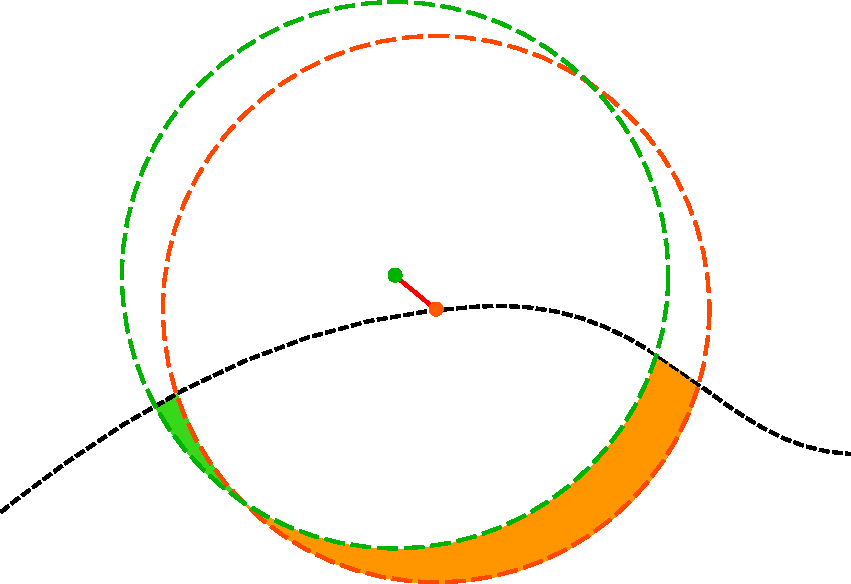
\includegraphics[width=5cm]{figures/momentsPerturbation}
      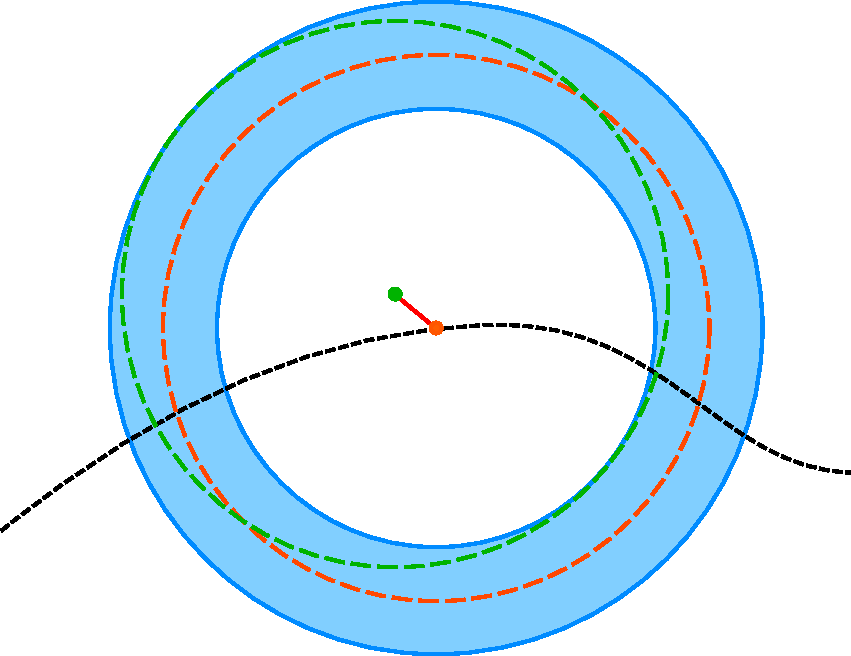
\includegraphics[width=5cm]{figures/momentsPerturbation2}
    \end{center}
    \caption[Illustration du \RefLemma{lem:moments-ball-position-error}.]{Illustration du \RefLemma{lem:moments-ball-position-error}.}
    \label{fig:moments-perturb}
\end{figure}
\todoJeremy{Pb avec la figure}
%
En décomposant $\Shape$ en fonction de deux boules de rayon R, centrées en $\vx$
et $\vx + \vt$ (voir \RefFigure{fig:moments-perturb}), nous avons :
%
\begin{align}
  \Mom{pqs}&(\Ball{R}{\vx+\vt} \cap \Shape ) - \Mom{pqs}(\Ball{R}{\vx} \cap \Shape ) \\
    &= \Mom{pqs}( (\Ball{R}{\vx+\vt} \setminus \Ball{R}{\vx}) \cap \Shape ) \\
    & \quad - \Mom{pqs}( (\Ball{R}{\vx} \setminus \Ball{R}{\vx+\vt}) \cap \Shape )
\end{align}
%
Comme :
%
\begin{equation}
  \emptyset \neq Y_1 \subset Y_2 \subset \R^3 \Implies \sup_{ Y \subset Y_1} \left | \Mom{pqs}(Y) \right| \le \sup_{Y \subset Y_2} \left| \Mom{pqs}(Y)\right |,
\end{equation}
%
et avec la propriété d'additivité des intégrales, nous avons :
%
\begin{align}
  |\Delta(\vt)| &= |\Mom{pqs}( (\Ball{R}{\vx+\vt} \ominus \Ball{R}{\vx}) \cap \Shape )| \\
  &\le \sup_{Y \subset (\Ball{R}{\vx+\vt} \ominus \Ball{R}{\vx}) \cap \Shape} |\Mom{pqs}(Y)|\\
  &\le \sup_{Y \subset \Ball{R}{\vx+\vt} \ominus \Ball{R}{\vx}} |\Mom{pqs}(Y)|\\
  &\le \sup_{Y \subset \Ball{R+t}{\vx} - \Ball{R-t}{\vx}} |\Mom{pqs}(Y)|.
\end{align}
%
Pour une meilleure lisibilité, nous noterons $S_{R,t}(\vx) \EqDef
\Ball{R+t}{\vx} \setminus \Ball{R-t}{\vx}$. Nous couvrons alors la différence
entre les deux boules centrées en des points différents ($\Ball{R}{\vx+\vt}
\ominus \Ball{R}{\vx}$) par la différence entre deux boules de même centre mais
de rayons différents ($S_{R,t}(\vx)$). Ceci est représenté
en bleu sur la \RefFigure{fig:moments-perturb}, correspond à un anneau en 2D de
largeur $2t$. Il s'agit évidemment d'une borne supérieure épaisse, mais les
ordres de perturbations sont les mêmes.
%
\textbf{\\Moment d'ordre zéro.\quad}
%
Pour le moment d'ordre zéro, nous utilisons simplement le volume de la boule :
%
\begin{align}
  \sup_{Y \subset S_{R,t}(\vx)} |\Mom{000}(Y)|
  &= \Mom{000}( S_{R,t}(\vx) ) \\
  &= \frac{4\pi}{3}(R+t)^3 - \frac{4\pi}{3}(R-t)^3 \\
  &= \frac{4\pi}{3}(6R^2t+2t^3)=O(tR^2).
\end{align}
%
\textbf{\\Moments du premier ordre.\quad}
%
Pour les moments du premier ordre, nous translatons la forme à l'origine du
repère et nous utilisons le résultat précédent ainsi que le fait que le
$100$-moment centré est maximisé pour la demi-boule à valeur de $x_1$ positive
(que nous noterons $\HalfBall{R}{\vx}$)\footnote{Rappelons que $x_i$ est la
$i$ème composante de $\vx$.} :
%
\begin{align}
  \sup_{Y \subset S_{R,t}(\vx)} |\Mom{100}(Y)|
  &\le \sup_{Y \subset S_{R,t}(\mathbf{0})} |\Mom{100}(Y)| + |x_1|\cdot\Mom{000}(Y)\nonumber \\
  &= \Mom{100}( \HalfBall{R+t}{\mathbf{0}} - \HalfBall{R-t}{\mathbf{0}} ) + O(|x_1|tR^2) \nonumber \\
  &= 2\pi(R^3t +Rt^3) + O( (\| \vx \|_\infty) tR^2) \nonumber \\
  &= O(tR^3) + O(\| \vx \|_\infty tR^2).
\end{align}
%
\textbf{\\Moments du second ordre.\quad}
%
Pour les moments du second ordre, nous translatons également la forme à
l'origine du repère, puis nous utilisons les deux résultats précédents ainsi que
le fait que le $200$-moment est maximisé pour la boule :
%
\begin{align}
  \sup_{Y \subset S_{R,t}(\vx)} |\Mom{200}(Y)| &
  \le \sup_{Y \subset S_{R,t}(\mathbf{0})} |\Mom{200}(Y)| + 2|x_1|\cdot |\Mom{100}(Y)| + x_1^2\cdot\Mom{000}(Y) \nonumber \\
  & = \Mom{200}(S_{R,t}(\mathbf{0})) + \|\vx\|_\infty (O(tR^3) + O(\|\vx\|_\infty tR^2))+  \|\vx\|_\infty^2 O(tR^2) \nonumber \\
  & = O(tR^4) +O(\|\vx\|_\infty tR^3) +O(\|\vx\|_\infty^2 tR^2)
\end{align}
%
Les autres moments sont prouvés de la même façon.
%
\end{proof}
%
\paragraph{Convergence asymptotique des matrices de covariances digitales}
%
Avec le \RefLemma{lem:covariance-translation-invariant} et le
\RefLemma{lem:moments-ball-position-error}, nous pouvons facilement prouver la
convergence asymptotique des matrices de covariances digitales. Le théorème
suivant établie la convergence lorsque la matrice de covariance est calculée sur
le même point $\vy$, et le suivant établiera sa convergence asymptotique sur le
bord digital de la forme.
%
\begin{theorem}[Convergence de la matrice de covariance digitale.]
  \label{thm:conv-cov-matrix}
%
  Soit $\Shape$ un domaine compact de $\R^d$. Alors, il existe une constance
  $h_0$ telle que pour tout pas de discrétisation $0 < h < h_0$, pour tout $\vy
  \in \R^3$, pour un rayon $R \ge h$, nous avons\footnote{$\mu_i \ge 1$ d'après l'\RefEquation{eq:MomentsByCounting-conv}} :
%
  \begin{equation}
    \left \| \DCov{h}( \Ball{R/h}{\vy/h} \cap  \DSh ) - \Cov( \Ball{R}{\vy} \cap \Shape )\right \| \le \sum_{i=0}^2 O(R^{5-\mu_i}h^{\mu_i}).
  \end{equation}
%
  La constance cachée derrière le terme en grand « O » ne dépend pas de la
  taille de la forme ni de sa géométrie. $\|\cdot\|$ est la norme spectrale des
  matrices.
%
\end{theorem}
\begin{proof}
%
  Afin de faciliter la lecture, nous noterons $A \EqDef \Ball{R}{\vy} \cap
  \Shape$ et $A_h \EqDef \Ball{R/h}{\vy/h} \cap \DSh = \DigF{\Ball{R}{\vy} \cap
  \Shape}{h}$ (au sens de la discrétisation de Gauss). Nous commençons par
  translater les ensembles $A$ et $A_h$ centrés en $\vy$ vers l'origine du
  repère. Nous devons alors utiliser un vecteur qui prend compte de la
  discrétisation puisque nous décalons $A_h$ par le vecteur $\Rounded{\vy}{h}$
  (\comJeremy{vecteur entier} le plus proche de $\frac{\vy}{h}$) et nous
  décalons $A$ par le vecteur $h\Rounded{\vy}{h}$. Nous noterons alors
  $\tilde{A} \EqDef A -
  h\Rounded{\vy}{h}$ et $\tilde{A}_h \EqDef A_h - \Rounded{\vy}{h}$. Avec ces deux définitions et la propriété d'invariance des
  matrices de covariances digitales
  (\RefLemma{lem:covariance-translation-invariant}), nous obtenons :
%
  \begin{align}
    \DCov{h}( \Ball{R/h}{\vy/h} \cap \DSh )
    &= \DCov{h}( A_h )\\
    &= \DCov{h}\left( \tilde{A}_h + \Rounded{\vy}{h}\right )\\
    &= \DCov{h}( \tilde{A}_h )\\
    &= \DCov{h}( \DigF{\tilde{A}}{h} ). \label{eq:DigitalCovarianceMatrix-conv-proof1}
  \end{align}
%
  La dernière égalité vient du fait que $\tilde{A}_h = \DigF{A}{h} -
  \Rounded{\vy}{h} = \DigF{A - h\Rounded{\vy}{h}}{h} = \DigF{\tilde{A}}{h}$.
%
  Nous faisons de même avec la matrice de covariance continue :
%
  \begin{align}
    \Cov( \Ball{R}{\vy} \cap \Shape )
    &= \Cov( A ) \\
    &= \Cov\left( \tilde{A} + h\Rounded{\vy}{h} \right) \\
    &= \Cov( \tilde{A} ). \label{eq:DigitalCovarianceMatrix-conv-proof2}
  \end{align}
%
  Alors, nous pouvons réécrire l'erreur d'estimation de la matrice de covariance
  digitale comme :
%
  \begin{align}
    \| \DCov{h}( \Ball{R/h}{\vy/h} \cap \DSh ) - \Cov( \Ball{R}{\vx} \cap \Shape ) \|
    = \| \DCov{h}( \DigF{\tilde{A}}{h} ) - \Cov( \tilde{A} ) \|. \label{eq:DigitalCovarianceMatrix-conv-proof3}
  \end{align}
%
  Détaillons maintenant $\DCov{h}( \DigF{\tilde{A}}{h} )$ :
%
  \begin{equation}
    \DCov{h}( \DigF{\tilde{A}}{h} )
    = \left [
    \begin{array}{ccc}
      \DMom{200}{h}(\tilde{A}_h) & &\\
      & \ddots & \\
    \end{array}
    \right ]% \nonumber \\ &
    - \frac{1}{\DMom{000}{h}(\tilde{A}_h)}
    \left [ \begin{array}{c}
      \DMom{100}{h}(\tilde{A}_h) \\ \vdots
    \end{array} \right ]
    \otimes
    \left [ \begin{array}{c}
      \DMom{100}{h}(\tilde{A}_h) \\ \vdots
    \end{array} \right ]^T.
  \end{equation}
%
  En utilisant les résultats de l'\RefEquation{eq:MomentsOnUnitaryBall-conv},
  nous obtenons :
%
\begin{align}
  \DCov{h}( \DigF{\tilde{A}}{h} )
  &= \left [
  \begin{array}{ccc}
    \Mom{200}(\tilde{A}) + O(R^{5 - \mu_2} h^{\mu_2}) & &\\
    & \ddots & \\
  \end{array}
  \right ] \nonumber \\
  & \quad- \frac{1}{\Mom{000}(\tilde{A}) + O(R^{3 - \mu_0} h^{\mu_0})}
  \left [ \begin{array}{c}
    (\Mom{100}(\tilde{A}) + O(R^{4 - \mu_1} h^{\mu_1}))^2 \\ \vdots
  \end{array} \right ].
\end{align}
%
  Il est à noter que les constantes dans les termes en grand « O » sont
  indépendantes de $\Shape$ grâce à la normalisation. La précedente équation
  nous donne $\Cov( \tilde{A} )$ et des termes d'erreurs sur les moments. Nous
  allons alors chercher les bornes supérieures de ces moments dans le calcul de
  $\DCov{h}( \DigF{\tilde{A}}{h} )$ en sachant que le rayon $R$ est supérieur à
  $h$ et puisque $\tilde{A}$ n'est pas vide et est proche de l'origine, nous
  pouvons alors utiliser les
  \RefEquations{eq:ball-moment-1}{eq:ball-moment-1bis} du
  \RefLemma{lem:moment-ball} pour l'ensemble $\tilde{A} \subset \Ball{R}{t}$,
  pour les points $\vt = \vx - h\frac{\vx}{h}$, en sachant que $||\vt||_\infty
  \le \frac{h}{2}$. Nous obtenons alors :
  %
  \begin{equation}
    \DCov{h}( \DigF{\tilde{A}}{h} ) = \Cov(\tilde{A}) + O(R^{5-{\mu_2}}h^{\mu_2}) + O(R^{5-{\mu_0}}h^{\mu_0}) + O(R^{5-{\mu_1}}h^{\mu_1}).
  \end{equation}
  %
  Puisque $\Cov(\tilde{A})=\Cov(A-h\Rounded{x}{h})=\Cov(A)$ grâce à la propriété d'invariance à la translation des matrice de covariance du \RefLemma{lem:covariance-translation-invariant} :
  %
  \begin{equation}
    \DCov{h}( \DigF{\tilde{A}}{h} ) = \Cov(A) + O(R^{5-{\mu_2}}h^{\mu_2}) + O(R^{5-{\mu_0}}h^{\mu_0}) + O(R^{5-{\mu_1}}h^{\mu_1}).
  \end{equation}
%
\end{proof}
%
Comme pour le calcul de la courbure 2D ou courbure moyenne 3D, afin d'obtenir un
résultat de convergence asymptotique, nous devons placer notre estimateur
digital sur le bord digital de la forme, ajoutant une erreur de positionnement.
Cela équivaut à estimer les moments à une position $\vx + \vt$, et pour cela
nous allons nous servir des précédents lemmes.
%
\begin{theorem}[Convergence asymptotique de la matrice de covariance digitale]
\label{thm:multigrid-conv-cov-matrix}
%
  Soit $\Shape$ un domaine compact de $\R^3$. Alors, il existe une constance
  $h_0$ telle que pour tout pas de discrétisation $0 < h < h_0$, pour tout $\vx
  \in \R^3$, pour un rayon $R \ge h$, nous avons\footnote{$\mu_i \ge 1$ d'après l'\RefEquation{eq:MomentsByCounting-conv}} :
%
  \begin{align}
    &\forall 0 < h < h_0, \quad \forall \vx \in \Bd{\Shape}, \quad
    \forall \hat{\vx} \in \Bd{\Body{\DSh}{h}} \text{~avec~} \| \hat{\vx} -\vx\|_\infty \le h, \nonumber \\
    &\left\| \DCov{h}( \Ball{R/h}{\hat{\vx}/h} \cap  \DSh ) - \Cov( \Ball{R}{\vx} \cap \Shape )\right \|\le O(\|\vx-\hat{\vx}\| R^4) + \sum_{i=0}^2 O(R^{5-\mu_i}h^{\mu_i}),
  \end{align}
  %
  La constance cachée derrière le terme en grand « O » ne dépend pas de la
  taille de la forme ni de sa géométrie. $\|\cdot\|$ est la norme spectrale des
  matrices.
  %
\end{theorem}
\begin{proof}
  %
  %Pour plus de facilité de lecture, nous allons noter $A \EqDef \Ball{R}{\vx}
  %\cap \Shape$ et $A_h \EqDef \Ball{R/h}{\hat{\vx}/h} \cap \DSh = \DigF{\Ball{R}{\hat{\vx}}
  %\cap \Shape}{h}$.
  Le fait que $\| \vx - \hat{\vx} \|_\infty \le h \le R$ implique que
  $\Ball{R}{\vx} \cap \Shape$ et $\Ball{R}{\hat{\vx}} \cap \Shape$ ne sont pas
  vides. Nous séparons alors la différence des matrices en deux parties :
  %
  \begin{align}
  &\| \DCov{h}( \Ball{R/h}{\hat{\vx}/h} \cap  \DigF{\Shape}{h} ) - \Cov( \Ball{R}{\vx} \cap \Shape ) \| \\ \nonumber
  & \quad \le  \| \DCov{h}( \Ball{R/h}{\hat{\vx}/h} \cap  \DigF{\Shape}{h} ) - \Cov( \Ball{R}{\hat{\vx}} \cap \Shape ) \|
  + \| \Cov( \Ball{R}{\hat{\vx}} \cap \Shape ) - \Cov( \Ball{R}{\vx} \cap \Shape ) \|.
 \end{align}
  %
  Nous avons borné le premier terme par $\sum_{i=0}^2 O(R^{5-\mu_i}h^{\mu_i})$
  dans le \RefTheorem{thm:conv-cov-matrix} si nous l'appliquons au point
  $\hat{\vx}$. Pour le second terme, nous définissons $\vt \EqDef \hat{\vx} -
  \vx$, $t \EqDef \| \vt \|_2$, and $\Shape' \EqDef \Shape - \vx$. Nous
  utilisons alors la propriété d'invariance à la translation des matrices de
  covariance (\RefLemma{lem:covariance-translation-invariant}) afin de déplacer
  les matrices à l'origine du repère :
  %
  \begin{align}
    &\| \Cov( \Ball{R}{\hat{\vx}} \cap \Shape ) - \Cov( \Ball{R}{\vx} \cap \Shape )\|
    = \| \Cov( \Ball{R}{\vx + \vt} \cap \Shape ) - \Cov( \Ball{R}{\vx} \cap \Shape )\| \\
    & \quad = \| \Cov( \Ball{R}{\vx + \vt} \cap \Shape - \vx ) - \Cov( \Ball{R}{\vx} \cap \Shape - \vx )\| \\
    & \quad = \| \Cov( (\Ball{R}{\vx + \vt} - \vx) \cap (\Shape - \vx) ) - \Cov( (\Ball{R}{\vx} - \vx) \cap (\Shape - \vx) )\| \\
    & \quad = \| \Cov( \Ball{R}{\vt} \cap (\Shape - \vx) ) - \Cov( \Ball{R}{\mathbf{0}} \cap (\Shape - \vx) )\| \\
    & \quad = \| \Cov( \Ball{R}{\vt} \cap \Shape' ) - \Cov( \Ball{R}{\mathbf{0}} \cap \Shape' )\|.
  \end{align}
  %
  Nous appliquons maintenant le \RefLemma{lem:moments-ball-position-error} pour
  les différents moments qui interviennent dans la matrice de covariance $\Cov$.
  Pour une facilité de lecture, nous noterons $Y_{\vt}$ l'ensemble
  $\Ball{R}{\vt} \cap \Shape'$ et $Y_{\mathbf{0}}$ l'ensemble
  $\Ball{R}{\mathbf{0}} \cap \Shape'$.
  %
  \begin{align}
   \| \Cov( Y_{\vt} ) - \Cov(Y_{\mathbf{0}})\|
   &= \left\| \left\lbrack \begin{array}{cc}
       \Mom{200}(Y_{\vt}) - \Mom{200}(Y_{\mathbf{0}}) & \\
       & \ddots
     \end{array} \right\rbrack
   \right. \nonumber\\
  & - \frac{1}{\Mom{000}(Y_{\vt})}
   \left\lbrack \begin{array}{c}
     \Mom{100}(Y_{\vt}) \\
     \vdots
   \end{array} \right\rbrack
   \otimes
   \left\lbrack \begin{array}{c}
     \Mom{100}(Y_{\vt}) \\
     \vdots
   \end{array} \right\rbrack^T
   \nonumber\\
  & \left.
   + \frac{1}{\Mom{000}(Y_{\mathbf{0}})}
   \left\lbrack \begin{array}{c}
     \Mom{100}(Y_{\mathbf{0}}) \\
     \vdots
   \end{array} \right\rbrack
   \otimes
   \left\lbrack \begin{array}{c}
     \Mom{100}(Y_{\mathbf{0}}) \\
     \vdots
   \end{array} \right\rbrack^T
   \right\|.
  \end{align}
  %
  La matrice $\Cov( Y_{\vt} ) - \Cov(Y_{\mathbf{0}})$ contient alors la
  différece des moments géométriques du second ordre comme par exemple $
  \Mom{200}(Y_{\vt}) - \Mom{200}(Y_{\mathbf{0}})$ et des quantités de la forme
  de $\Delta \EqDef \frac{\Mom{100}(Y_{\vt})^2}{\Mom{000}(Y_{\vt})} -
  \frac{\Mom{100}(Y_{\mathbf{0}})^2}{\Mom{000}(Y_{\mathbf{0}})}$ si on décompose
  les termes de droite. D'après le \RefLemma{lem:moments-ball-position-error},
  nous savons que les erreurs des moments du second ordre sont bornées en $O(t
  R^4)$. Pour borner $\Delta$, nous savons déjà $|\Mom{000}(Y_{\mathbf{t}}) -
  \Mom{000}(Y_{\mathbf{0}})| = \pi R^2(t+O(t^2)+O(tR^2))$ en utilisant le
  \RefTheoremFake{7}{Pottmann2009}. Alors, nous obtenons :
  %
  \begin{align}
    \Delta &= \frac{\Mom{100}(Y_{\vt})^2}{\Mom{000}(Y_{\mathbf{0}}) + O(tR^2)} -
    \frac{\Mom{100}(Y_{\mathbf{0}})^2}{\Mom{000}(Y_{\mathbf{0}})}\\
    &= O(tR^2)\frac{\Mom{100}(Y_{\vt})^2}{\Mom{000}(Y_{\mathbf{0}})^2} +
    \frac{\Mom{100}(Y_{\vt})^2 - \Mom{100}(Y_{\mathbf{0}})^2}{\Mom{000}(Y_{\mathbf{0}})}\,.
  \end{align}
  %
  Puisque $\frac{a}{b+O(x)}=\frac{a}{b}+\frac{a}{b^2}O(x)$, $a^2-b^2=(a-b)(a+b)$
  et en utilisant de nouveau le \RefLemma{lem:moments-ball-position-error}, nous
  avons :
  %
  \begin{align*}
    \Delta
    &= O(tR^4) + (\Mom{100}(Y_{\vt}) + \Mom{100}(Y_{\mathbf{0}}))\frac{\Mom{100}(Y_{\vt}) - \Mom{100}(Y_{\mathbf{0}})}{\Mom{000}(Y_{\mathbf{0}})} \\
    &= O(tR^4) + (O(tR^3)+O(R^4))\frac{\Mom{100}(Y_{\vt}) - \Mom{100}(Y_{\mathbf{0}})}{\Mom{000}(Y_{\mathbf{0}})}
  \end{align*}
  %
  Nous utilisons le \RefLemma{lem:moments-ball-position-error} et le fait que
  puisque $t < R$ nous avons $\Mom{000}(Y_{\mathbf{0}}) = O(R^3)$, nous avons :
  %
  \begin{equation}
    \Delta = O(tR^4) + (O(tR^3)+O(R^4))\frac{O(tR^3)}{\Mom{000}(Y_{\mathbf{0}})} = O(tR^4).
  \end{equation}
  %
  Les mêmes bornes sont trouvés pour tous les termes de la matrice. Lorsqu'on
  les rassemble toutes, nous obtenons le résultat du théorème.
  %
  \end{proof}
%

\todoInlineJeremy{-------------------------------}
% \todoInlineJeremy{-------------------------------}
% \todoInlineJeremy{-------------------------------}
% \todoInlineJeremy{-------------------------------}
% \todoInlineJeremy{-------------------------------}
% \todoInlineJeremy{-------------------------------}
% \todoInlineJeremy{-------------------------------}
% \todoInlineJeremy{-------------------------------}
% \todoInlineJeremy{-------------------------------}
% \todoInlineJeremy{-------------------------------}
% \vxH \in \Bd{\Body{\DSh}{h}}


% \begin{definition}
%   \begin{equation}
%     \hat{\kappa}^{i}(Z,p) \EqDef \frac{1}{h} \left( \frac{6(\hat{\lambda}_2
%      - 3\hat{\lambda}_1)}{\pi {{R_d}}^6} + \frac{8}{5{{R_d}}} \right).
%   \end{equation}
%   \label{}
% \end{definition}
\begin{definition}{\textbf{(Estimateurs de courbures principales discrètes 3D $\PrincCurvH{i}{}(Z,p)$).}}
  \label{def:ii-3d-princ}
  Let $\DigShape$ be a digital shape, $\vx$ some point of $\R^3$ and $h>0$ a
  grid step. For $R\ge h$, we define the {\em integral principal
    curvature estimators $\PrincCurvH{1}{R}$ and $\PrincCurvH{2}{R}$} of
  $\DigShape$ at point $\vy \in \R^3$ and step $h$ as
\begin{eqnarray}
  \PrincCurvH{1}{R}(\DigShape,\vy,h) &=& \frac{6}{\pi R^6}(\hat{\lambda}_2 - 3\hat{\lambda}_1) + \frac{8}{5R},\\
  \PrincCurvH{2}{R}(\DigShape,\vy,h) &=& \frac{6}{\pi R^6}(\hat{\lambda}_1 - 3\hat{\lambda}_2) + \frac{8}{5R},
\end{eqnarray}
where $\hat{\lambda}_1$ and $\hat{\lambda}_2$ are the two greatest
eigenvalues of $\hat{J}(\Ball{R/h}{\frac{1}{h} \cdot y} \cap \DigShape, h ))$.
\end{definition}

We recall the following result of matrix perturbation theory %\cite{Bauer:1960,stewart1990matrix,bhatia1997matrix}:
\begin{theorem}{\textbf{(Lidskii-Weyl inequality).}}
  \label{thm:lidskii-weyl}
  If $\lambda_i(B)$ denotes the ordered eigenvalues of some symmetric
  matrix $B$ and $\lambda_i(B+E)$ the ordered eigenvalues of some
  symmetric matrix $B+E$, then $\max_{i}| \lambda_i(B) -
  \lambda_i(B+E)| \le \|E\|$.
\end{theorem}


% Convergence des estimateurs de courbures principales discrètes 3D $\hat{\kappa}^{i}(Z,p)$ :
% \begin{theorem}
%   \begin{equation}
%     \hat{\kappa}^i_{R}(\DSh,p) = \PrincCurv{1}(X,x) + O(h^{\frac{1}{3}}).
%   \end{equation}
%   \label{theo:ii-3d-princ-conv}
% \end{theorem}
\begin{theorem}{\textbf{(Uniform convergence of principal curvature estimators $\PrincCurvH{1}{R}$ and $\PrincCurvH{2}{R}$ along $\hBd{h} \Shape$).}}
  \label{theo:ii-3d-princ-conv}
  Let $\Shape \in \Shapes$. For $i \in \{1,2\}$, recall that
  $\PrincCurv{i}(\Shape,\vx)$ is the $i$-th principal curvature of $\Bd{\Shape}$ at
  boundary point $\vx$. Then, there exist  positive constants $h_\Shape,k,K$ such that, for any $h \le
  h_\Shape$, setting $R=k h^{\frac{1}{3}}$, we have
  \begin{align*}
     &\forall \vx \in \partial \Shape, \forall \hat{\vx} \in \hBd{h}\Shape,\nonumber\\
     &\| \hat{\vx} - \vx\|_\infty \le h \Implies |
     \PrincCurvH{i}{R}(\DSh,\hat{\vx},h) - \PrincCurv{i}(\Shape,\vx) | \le K
     h^{\frac{1}{3}}.
  \end{align*}
\end{theorem}


\subsection{Estimation de la courbure par intégration surfacique de la sphère}
\subsubsection{Analyse euclidienne de l'intégration surfacique de la sphère, et relation à la courbure}
\paragraph{Estimation par aire de patch de surface}
\paragraph{Estimation par aire de surface de sphère}

\section{Estimateurs de normales}
\subsection{État de l'art}
\subsection{Estimation par aire/volume de sphère}
